\documentclass[12pt,twoside]{report}

\author{Oliver Kohlbacher, Heiko Klein,\\ Andreas Kerzmann}
\title{
	\begin{center}
		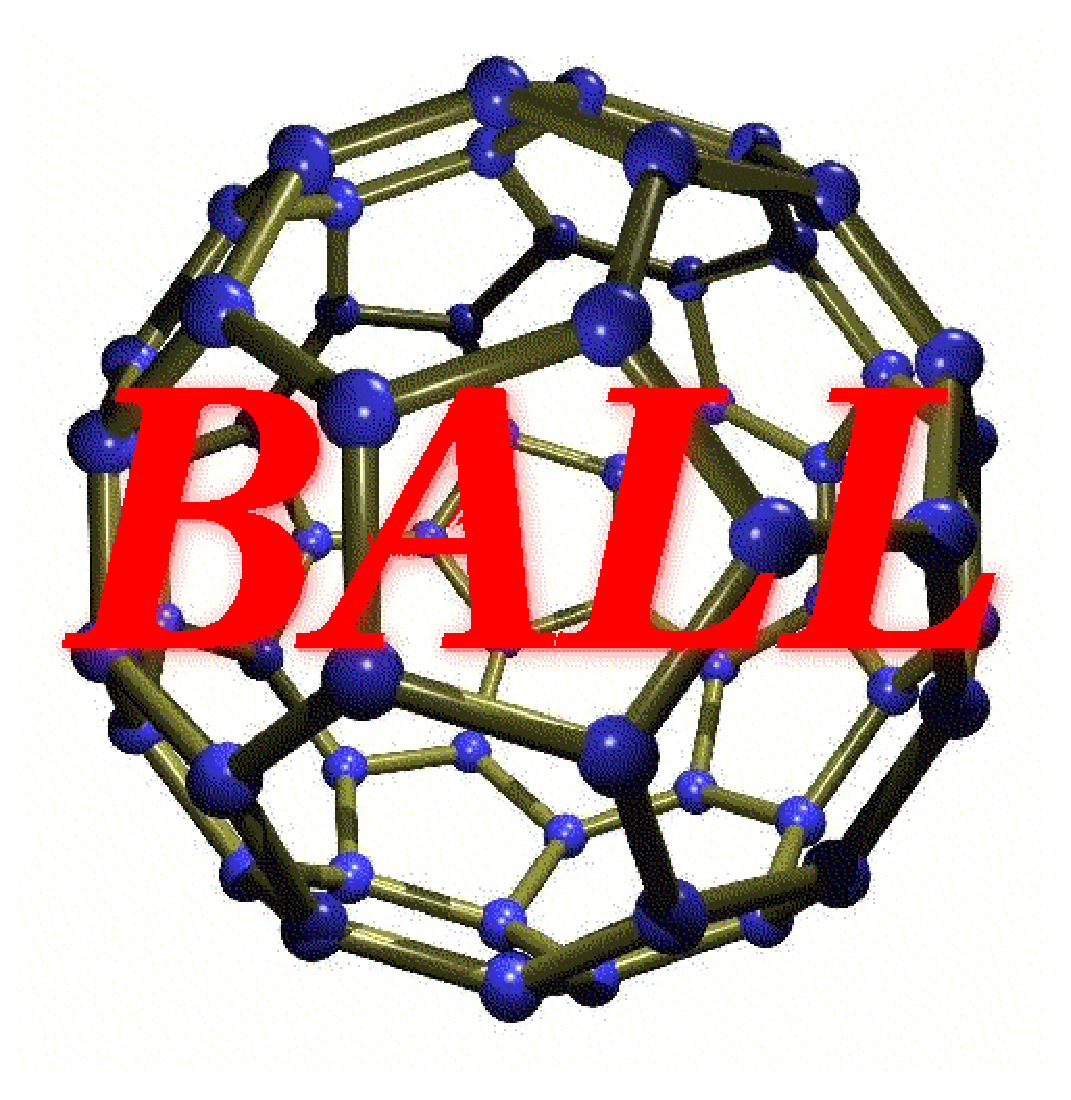
\includegraphics[width=10cm]{logo.eps}
	\end{center}
	\Huge BALL\\ 
	\Large A Tutorial
}

\usepackage{longtable}
%-----------------------------------------
% used packages
%-----------------------------------------
\usepackage{a4}
% use A4 paper

%\usepackage[draft]{graphicx}
\usepackage{graphicx}
% use graphics package

\usepackage{times}
% use postscript fonts

\usepackage{psboxit}
\newcommand{\graybox}[1]{\psboxit{box .85 setgray fill}{\fbox{#1}}}
% display gray shaded boxes using postscript commands
%


%-----------------------------------------
% quote environment for quatations
%-----------------------------------------
% in part stolen from LaTeX companion
\usepackage{ifthen}
\newsavebox{\QuoteNameBox}
\newenvironment{Quote}[1]%
	{%
		\sbox{\QuoteNameBox}{{\it #1}}%
		\begin{list}{}{%
			\setlength{\rightmargin}{\leftmargin}}%
				\item[]``\ignorespaces}%
	{\unskip''\hfill \usebox{\QuoteNameBox}\end{list}}


\usepackage{changebar}
% This package defines the two commands \cbstart and \cbend. It then displays a
% bar between the start and the end command

\usepackage{color}
% This package allows the coloring of text (e.g. in an ipe minipage)

\usepackage{float}
% the float package allows a better placement of all floats (figures,tables) or
% even new floats it allows the following kinds of boxes:
% \shadowbox, \doublebox, \ovalbox, \Ovalbox

\makeatletter
	\renewcommand{\@makecaption}[2]{
		\vspace{3pt}
		\noindent{\color{blue}\rule{\textwidth}{1pt}}\par
		\noindent{\small{\sffamily #1:}\hspace{5pt}\itshape #2\par}
		\vspace{5pt}
	}
\makeatother
% 
%  create a fancy float caption: 
%    - blue rule under the float
%    - the figure text set in sans serif
%    - the caption text in italics

\setcounter{topnumber}{1}
\setcounter{bottomnumber}{1}
%
%  	some settings for the floats: just on float at the
%		top of a page and on at the bottom

	
%-----------------------------------------
% Font definitions 
%-----------------------------------------

\usepackage{amsfonts}
\usepackage{amsmath}
\usepackage{amsthm}
\usepackage{amssymb}

%-----------------------------------------
% Textlayout 
%-----------------------------------------

\newcommand{\clearemptydoublepage}{\newpage{\pagestyle{empty}\cleardoublepage}}

%\usepackage{a4wide}
\setlength{\textheight}{21cm}
\setlength{\textwidth}{14.5cm}
\setlength{\oddsidemargin}{10mm}
\setlength{\evensidemargin}{2mm}
\setlength{\topmargin}{0mm}
%\setlength{\marginparsep}{5mm}
%\setlength{\marginparwidth}{2cm}
%\renewcommand{\baselinestretch}{1.21}
\large\normalsize

%-----------------------------------------
% some shorthands
%-----------------------------------------

\providecommand{\R}{\mathbb R}
\providecommand{\Q}{\mathbb Q}
\providecommand{\N}{\mathbb N}
\providecommand{\Z}{\mathbb Z}

%-----------------------------------------
% redefinitions of sectioning comands
%-----------------------------------------

\usepackage{fancyheadings}
% allows you an easy adaption of the headings

\usepackage{fancybox}
% you can use shaded boxes e.g. for figures it allows the following kinds of boxes:
% \shadowbox, \doublebox, \ovalbox, \Ovalbox

\addtolength{\headrulewidth}{0.2pt}
\addtolength{\footrulewidth}{0.6pt}
\addtolength{\headwidth}{1cm}
\addtolength{\footskip}{10mm}
\addtolength{\headsep}{5mm}
\addtocounter{secnumdepth}{2}
\setcounter{tocdepth}{3}
\setcounter{secnumdepth}{3}

\renewcommand{\chaptermark}[1]{\hfill\markboth{#1}{}\hfill}
\renewcommand{\sectionmark}[1]{\hfill\markright{\thesection\ #1}\hfill}
\lhead{}
\rhead{}
\chead[\fancyplain{}{\textrm{\leftmark}}]%
      {\fancyplain{}{\textrm{\rightmark}}}
\cfoot{}
\rfoot[\fancyplain{}{}]{\fancyplain{}{\bfseries\thepage}}
\lfoot[\fancyplain{}{\bfseries\thepage}]{\fancyplain{}{}}


% the \chapter ...
\makeatletter
%\renewcommand\thesection 			{{\sffamily\thechapter.\@arabic\c@section}}
%\renewcommand\thesubsection   {{\sffamily\thesection.\@arabic\c@subsection}}
%\renewcommand\thesubsubsection{{\sffamily\thesubsection.\@arabic\c@subsubsection}}
\renewcommand{\@chapapp}{\sffamily}
%\renewcommand\section{\@startsection {section}{1}{\z@}%
%	{-3.5ex \@plus -1ex \@minus -.2ex}%
%	{2.3ex\@plus.2ex}%
%	{\normalfont\Large\sffamily\bfseries}
%}
%\renewcommand\subsection{\@startsection{subsection}{2}{\z@}%
%	{-3.25ex\@plus-1ex \@minus -.2ex}%
%	{1.5ex \@plus .2ex}%
%	{\normalfont\large\sffamily\bfseries}
%}
%\renewcommand\subsubsection{\@startsection{subsubsection}{3}{\z@}%
%	{-3.25ex\@plus-1ex \@minus -.2ex}%
%	{1.5ex \@plus .2ex}%
%	{\normalfont\normalsize\sffamily\bfseries}
%}
\makeatother

%-----------------------------------------
% macro for missing pieces
%-----------------------------------------
\usepackage{changebar}
\newcommand{\missing}[1]{
	\cbstart  % add a gray bar at the side of the page
	\message{^^JMISSING: #1^^J}
	\par\noindent\fbox{{\bf MISSING:} #1}\par
	\cbend
}

%-----------------------------------------
% rules for figures
%-----------------------------------------

\topfigrule
\botfigrule
\setlength{\shadowsize}{2pt}

%-----------------------------------------
% some shorthands
%-----------------------------------------

\usepackage{xspace}
% you should use \xspace in defining shorthands 
% e.g. \newcommand{\eg}{e.g., \xspace} \@ is for the correct spacing after punctuation

\newcommand{\eg}{{\it e.g.}\xspace}
\newcommand{\ie}{{\it i.e.}\xspace}
\newcommand{\ea}{{\it et al.}\xspace}
\newcommand{\etc}{{\it etc.}\xspace}
\def\CPP{C\raise.08ex\hbox{\tt ++}\xspace}


%-----------------------------------------
% the index
%-----------------------------------------
\usepackage{makeidx}

\newcommand{\Index}[1]{#1\index{#1}}
% prints the term and creates an index entry

\newcommand{\class}[1]{{\ttfamily{#1}}\index{#1@{\ttfamily{#1}}
(BALL~class)}\index{BALL!classes!#1@{\ttfamily{#1}}}}
% BALL class names are typeset in typewriter bold and indexed automatically:
%  - first with their class name
%  - then under BALL!classes!<classname>

\newcommand{\STLclass}[1]{{\ttfamily{#1}}\index{#1@{\ttfamily{#1}}
(STL~class)}\index{STL!#1 class@{\ttfamily{#1}}}}
% STL class names are typeset in typewriter bold and indexed automatically:
%  - first with their class name
%  - then under STL!<classname> class

\newcommand{\function}[1]{{\ttfamily{#1}}\index{#1@{\ttfamily{#1}}
(BALL~function)}\index{BALL!functions!#1@{\ttfamily{#1}}}}
% BALL function names are typeset in typewriter bold and indexed automatically:
%  - first with their name
%  - then under BALL!functions!<function name>

\newcommand{\method}[1]{{\ttfamily{#1}}\index{#1@{\ttfamily{#1}}
(method)}\index{BALL!functions!#1@{\ttfamily{#1}}}}
% method names are typeset in typewriter bold and indexed automatically:
%  - first with their name
%  - then under BALL!methods!<function name>

\newcommand{\attribute}[2]{{\ttfamily{#1}}\index{#1@{\ttfamily{#2}}
({\ttfamily #1} attribute)}\index{BALL!!#1!#2@{\ttfamily{#1}}}}
% attribute names are typeset in typewriter bold and indexed automatically:
%  - first with their name and (<class> attribute)
%  - then under BALL!<class>!<attribute>

\newcommand{\macro}[1]{{\ttfamily{#1}}\index{#1@{\ttfamily{#1}}
(BALL~macro)}\index{BALL!macros!#1@{\ttfamily{#1}}}}
% BALL macros names are typeset in typewriter bold and indexed automatically:
%  - first with their name
%  - then under BALL!macros!<macro name>

\newcommand{\namespace}[1]{{\ttfamily{#1}}\index{#1@{\ttfamily{#1}}
(BALL~namespace)}\index{BALL!namespaces!#1@{\ttfamily{#1}}}}
% BALL macros names are typeset in typewriter bold and indexed automatically:
%  - first with their name
%  - then under BALL!namespaces!<name>

\newcommand{\type}[1]{{\ttfamily{#1}}\index{#1@{\ttfamily{#1}}
(BALL~type)}\index{BALL!types!#1@{\ttfamily{#1}}}}
% BALL macros names are typeset in typewriter bold and indexed automatically:
%  - first with their name
%  - then under BALL!types!<macro name>

\newcommand{\file}[1]{
	{\ttfamily\mbox{#1}}
	\index{#1@{\ttfamily{#1}} (file)}
}
% BALL file names are typeset in typewriter bold and indexed automatically:
% with their name and "(file)" appended

\newcommand{\directory}[1]{
	{\ttfamily\mbox{#1}}
	\index{#1@{\ttfamily{#1}} (directory)}
}
% BALL directories are typeset in typewriter bold and indexed automatically:
% with their name and "(directory)" appended

\newcommand{\option}[1]{
	{\ttfamily\mbox{#1}}
	\index{configure!options!#1@{\ttfamily\mbox{#1}}}
}
% BALL file names are typeset in typewriter bold and indexed automatically:
% as configure/options/<name>"

\newcommand{\exception}[1]{{\ttfamily{#1}}\index{#1@{\ttfamily{#1}}
(BALL~class)}\index{BALL!exceptions!#1@{\ttfamily{#1}}}}
% BALL exceptions names are typeset in typewriter bold and indexed automatically:
%  - first with their name
%  - then under BALL!exceptions!<exception name>

\newcommand{\newtermdef}[1]{{\em #1}\index{#1!definition}}
% prints the term in italics and includes creates an index entry
% with the subentry "definition"

\newcommand{\newterm}[1]{{\em #1}\index{#1}}
% prints the term in italics and creates an index entry

\newcommand{\URL}[1]{{\bfseries\ttfamily\mbox{#1}}}
\newcommand{\email}[1]{{\bfseries\ttfamily\mbox{#1}}}

%--------------------------------------------
%  the style of embedded listings
%--------------------------------------------
\usepackage{listings}
% formatting of the listings
\lstset{
	%% we use ANSI C++
	language=[ANSI]C++,
%
	%% our tabs are always expanded to 2 blanks
	tabsize=2,
%
	%% the font size of the listing
	basicstyle=\small\ttfamily,
%
	%% make the listing as wide as \textwidth
	spread=-0.3cm,
%
	%% draw a line at the left of the listing
	frame=tlrb,
%
	%% captions appear at the bottom of the listing
	%captionpos=b,
%
	%% and make the corners of the frame round
	frameround=tttt,
%
	%% the label font
	labelstyle=\sffamily,
%
	%% line numbers for each line
	labelstep=0
}
\newcommand{\linelisting}{\lstinline[frame=,basicstyle=\small]}


%%
%%
%%     FAQ macros
%%
\newcounter{FAQcounter}
\newcounter{FAQseparatorCounter}
\setcounter{FAQcounter}{0}
\setcounter{FAQseparatorCounter}{0}
\newcommand{\FAQquestion}[1]{%
	\ifthenelse{\theFAQseparatorCounter=0}{}{\vspace{0.5mm}\begin{center}\rule{0.5\textwidth}{0.1pt}\end{center}\vspace{0.5mm}}%
	\stepcounter{FAQcounter}%
	\stepcounter{FAQseparatorCounter}%
	\noindent{\normalfont\bf\sffamily Question \theFAQcounter:} {\em #1 \par}%
}
\newcommand{\FAQanswer}[1]{\bigskip\noindent{\normalfont\bf\sffamily Answer:} #1\par}	
\newcommand{\FAQURL}[1]{\mbox{\tt #1}}
\newcommand{\FAQCategory}[1]{
	\par\vspace{0.5cm}
	\graybox{\hspace{-3pt}\makebox[\linewidth][c]{\normalfont\bf\sffamily\Large{#1}}}
	\par\vspace{0.6cm}
	\setcounter{FAQseparatorCounter}{0}
}

\pagestyle{fancyplain}
\sloppy
\makeindex

\begin{document}
\maketitle

\pagenumbering{roman}
\setcounter{page}{1}
\tableofcontents
\pagenumbering{arabic}
\setcounter{page}{1}


\chapter{Introduction}
\label{chapter:introduction}
BALL (Biochemical Algorithms Library) is an application framework for rapid
software prototyping in the field of Molecular Modeling.  This tutorial shall
help new users to make their first steps with BALL. It is {\em not} a full
documentation. For a full documentation, please refer to the \newterm{Reference
Manual}~\cite{BALL-RM} which can be obtained in HTML, PDF, or postscript format.

There are also several papers and technical reports published on
BALL~\cite{BKL99a,BKL99b,KL99} that give a cursory overview of its design
principles and illustrate its use in Rapid Software Prototyping.

An up to date version of BALL can be obtained from the website

\begin{enumerate}
  \item[] \URL{http://www.mpi-sb.mpg.de/BALL}
\end{enumerate}

\noindent 
as well as further documentation, bug reports, and changes.

The next section of this tutorial gives a short overview of the structure and
contents of BALL. Chapter \ref{chapter:getting-started} describes the
installation and related issues. In Chapter \ref{chapter:first-steps}, some
fundamental concepts and classes are explained. Finally, Chapter
\ref{chapter:faq} tries to answer the most frequently asked questions.

\section{Overview}
\index{BALL!overview}


The basis of all BALL classes is an extensive set of \newterm{foundation
classes}.  They provide generic implementations of advanced data structures
(\eg, trees, hash associative containers, hash grids, \etc), mathematical
objects (\eg, matrices, vectors, geometric objects), implementations of
\Index{design patterns}, object \Index{persistence}, and access to the
operating system (\eg, networking support, file handling).

The BALL \newterm{kernel} contains the molecular data structures for the
representation of atoms, bonds, molecules, proteins, \etc  The kernel classes
are implemented with the foundation classes and are carefully designed to
provide maximum extensibility and flexibility.
\begin{figure}[tb]
  \centering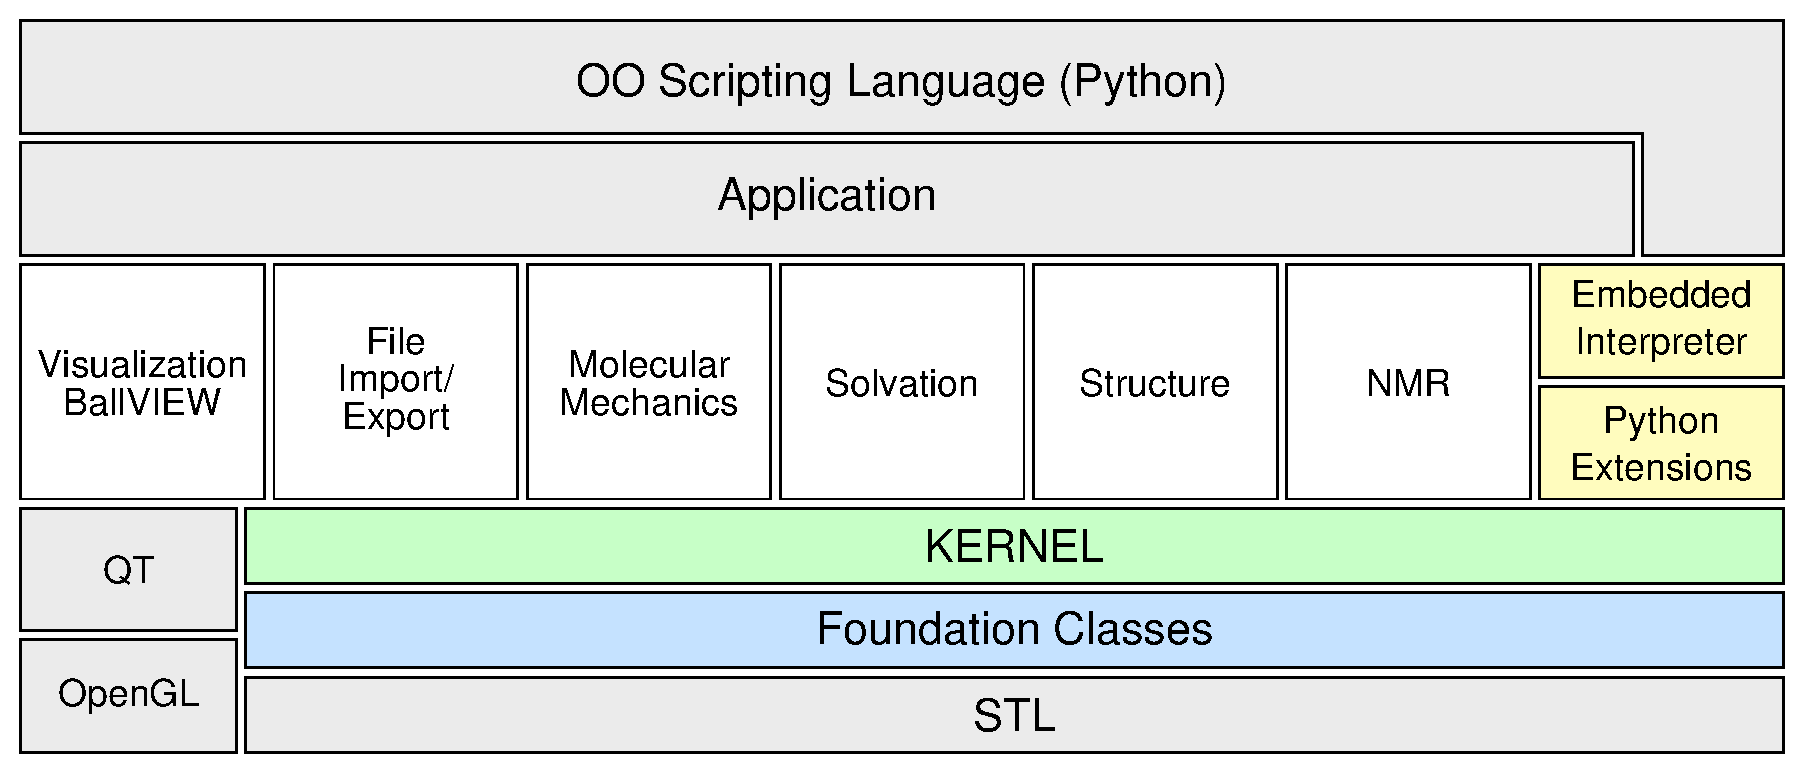
\includegraphics[width=\textwidth]{BALL_structure.eps}
  \caption{Overview of the structure of BALL}
  \label{fig:BALL_structure}
\end{figure}

The third layer of classes (on top of the foundation classes and the kernel)
provides the functionality required for applications. We call them
\newterm{basic components}. Each of these basic components is independent of
the other components.  We have implemented five basic components that cover
\Index{Molecular Mechanics}, file import/export, advanced \Index{solvation
methods}, structure analysis/comparison, and \Index{visualization}. These
areas were selected, because our main interest stems from the field of protein
docking. The Molecular Mechanics component does not only provide standard
force fields (AMBER~\cite{AMBER95}, CHARMM~\cite{BBO+83}), but also a generic
\Index{force field}.  This generic force field is a base class for all force
fields. It implements fundamental methods to manage parameter files, parameter
assignment, and atom type assignment, and defines a common interface for all
force fields. Thus, large portions of code may be reused for the
implementation of new force fields.  The file import/export component
implements general methods for efficient file handling, but also methods to
read and write the most common file formats used for molecular structures
(\eg, PDB, MOL2). The solvation component provides methods for calculating
solvation effects. The first method that accounts for solvation is the atomic
contact energy by Zhang {\it et al.}~\cite{ZVC+97}. The second approach that
we implemented is a numerical solver for the \Index{Poisson-Boltzmann} equation.  The
structure component contains algorithms to search for common structural motifs
in proteins, to map molecules onto each other, and to calculate solvent
accessible and solvent excluded surfaces of molecules. For the visualization
of the results, we designed \Index{BALLVIEW}, a class hierarchy that
visualizes BALL kernel objects with standard representations (ball and stick,
van der Waals, ribbons, surfaces, \etc). The visualization was implemented
using OpenGL and QT~\cite{QT}. Hence, it is highly portable and enables the
user to produce state-of-the-art graphical user interfaces with a minimum
effort.





\chapter{Getting Started}
\label{chapter:getting-started}
\section{System Requirements}

\subsection{Compiler}
\index{compiler}
  BALL requires an ANSI compliant \CPP compiler or GNU gcc
  (version above 2.95 or above).
  It has been successfully built and tested on the following platforms:
	\begin{itemize}	
   	\item Linux/x86 2.x using g\tt{++} 2.95.1 and 2.95.2
   	\item Solaris/SPARC 2.5.1, 2.6, 7 and 8 using g\tt{++} 2.95.2
   	\item Solaris/SPARC 7 using Kuck \& Associate (KAI) \CPP 3.4g
   	\item Solaris/SPARC 7 using SUN Workshop CC 6.0ea
   	\item Solaris/x86 2.6 using g\tt{++} 2.95.2
   	\item IRIX 6.5 using CC 7.3.1.1m
   	\item IRIX 6.5 using g\tt{++} 2.95.2
   	\item Compaq Tru64 Unix V5.0 using Compaq \CPP 6.2
 	\end{itemize}

\subsection{External software and libraries}
The compilation of the visualization component BALLVIEW also requires
the QT library (version 2.x) which is available from
\URL{http://www.troll.no/qt}.

If QT was not installed in one of the standard library paths or the
QT header files were not installed in one of the compiler's default
include directories, use "\option{--with-qt-libs}{\tt{}=DIR}" and
"\option{--with-qt-incl}{\tt{}=DIR}" as
options to configure (see Section \ref{section:building-ball}) to specify the paths
QT was installed to.\index{QT}
Please remember to compile also \file{libqgl.a}, which is one of the QT extensions
(to build \file{libqgl.a}, cd to {\tt\nobreak{\$QTDIR/extensions/opengl/src}} and type {\tt
make}).

QT also requires OpenGL. On platforms that do not provide OpenGL, MESA can
be used (e.g. Linux). Mesa is a 3-D graphics library with an API which is 
very similar to that of OpenGL. It can be obtained from \URL{http://www.mesa3d.org}.
\index{MESA}
If MESA is used, please call configure with the option "\option{--with-mesa}"

\section{Installation}
\label{section:building-ball}

Building BALL is very easy, but please read through this section carefully to
avoid any problems.  If all requirements stated above are met, BALL is built
by issuing the following commands in the directory {\tt BALL/source}:

\begin{lstlisting}{}
  ./configure
  make
\end{lstlisting}

The following sections give further details on the configuration of the library,
on the library files created, how to test the library, and how to build BALL 
applications.

\subsection{Configuring BALL}
\index{configure!usage}

"{\tt configure}" tries to gather as much information on your system as possible and 
then creates the necessary configuration files (\file{config.h},
\file{config.mak}, \file{common.mak}, and \file{Makefile}).
The configuration of BALL may be adapted to your needs and to your system
configuration from the command line by adding one or more of the options from
Table \ref{table:options}.
An overview of these options can also be obtained by executing "{\tt configure
--help}"

\begin{table}
\begin{center}
\begin{tabular}{lp{7cm}}\hline
  \option{--x-includes}{\tt{}=DIR}&        X include files are in DIR\\\vspace{3mm}

  \option{--x-libraries}{\tt{}=DIR}&       X library files are in DIR\\\vspace{3mm}

  \option{--enable-optimization}& optimize the library for speed, remove debug info\\\vspace{3mm}

  \option{--disable-debuginfo}& remove -g from the compiler flags (omit debug information)\\\vspace{3mm}

  \option{--disable-BALLVIEW}& disable the compilation of BALLVIEW, the visualization
												component\\\vspace{3mm}

  \option{--enable-64}&             build 64 bit objects (currently only supported for IRIX MipsPro 
                          compiler and SUNPro compiler)\\\vspace{3mm}

  \option{--with-compiler}{\tt{}=CXX}&     use CXX to compile BALL\\\vspace{3mm}

  \option{--with-cxxflags}{\tt{}=FLAGS}&   add \CPP compiler FLAGS to compile BALL\\\vspace{3mm}

  \option{--with-ldflags}{\tt{}=FLAGS}&    add FLAGS to the linker flags used to link the library and
        									                 applications\\\vspace{3mm}

  \option{--with-qt-incl}{\tt{}=DIR}&      QT header files are in DIR\\\vspace{3mm}

  \option{--with-qt-libs}{\tt{}=DIR}&      QT libraries are in DIR\\\vspace{3mm}

  \option{--with-opengl-incl}{\tt{}=DIR}&  OpenGL/Mesa header files are in DIR/GL\\\vspace{3mm}

  \option{--with-opengl-libs}{\tt{}=DIR}&  	OpenGL/Mesa libraries are in DIR/GL\\\vspace{3mm}

  \option{--with-mesa}&    				         	use MESA instead of OpenGL
								                  	       	If this option is specified, configure looks for libMesaGLU/libMesaGL.
									                         	If no libraries with these names are found, configure looks for
                  									       	libGLU and libGL.
									                         	This switch also add X11 libraries when trying to link agains the Mesa
									                         	libraries.\\\vspace{3mm}

  \option{--without-libxnet}&							 	use \Index{libsocket}/\Index{libnsl} for linking
										  										 	rather than \Index{libxnet}
							  	                         	this option is useful if some of your libraries (e.g. X11 libs)
									                         	were linked against libsocket/libnsl
																					 	\\\vspace{3mm}

  \option{--help}&                  display help information\\\hline
\end{tabular}
\end{center}
\caption{options for {\tt configure}}
\label{table:options}
\end{table}

For example, to compile BALL without the visualization component BALLVIEW,
specify 
\begin{lstlisting}{}
  configure --without-BALLVIEW
\end{lstlisting}

To include BALLVIEW using the QT installation in /opt/qt/lib and /opt/qt/include, specify

\begin{lstlisting}{}
  configure --with-qt-libs=/opt/qt/lib 
		--with-qt-incl=/opt/qt/include
\end{lstlisting}

If Mesa should be used (when compiling under Linux), the correct options might look
like this:

\begin{lstlisting}{}	
  configure --with-qt-libs=/opt/qt/lib 
		--with-qt-incl=/opt/qt/include --without-opengl
    --with-opengl-libs=/opt/mesa/lib 
		--with-opengl-incl=/opt/mesa/include
\end{lstlisting}

\subsection{Building the Libraries}

After the successful termination of configure, "make" builds the shared libraries.
There exist three different libraries:
\begin{center}
	\begin{tabular}{ll}
  	\file{libBALL.so}&     the main BALL library\\
  	\file{libVIEW.so}&     the visualization component BALLVIEW\\
	  \file{libMOLVIEW.so}&  the molecule--related stuff of BALLVIEW\\
	\end{tabular}
\end{center}

The latter two libraries are not built if "\option{--without-BALLVIEW}" is specified or configure
cannot find X libraries, OpenGL libraries, or QT libraries (and the respective headers).

It is also possible (although not recommended) to build the corresponding static libraries
\file{libBALL.a}, \file{libVIEW.a}, and \file{libMOLVIEW.a} using "{\tt make
staticlibs}".

\subsection{Installing the Libraries}

After compiling the libraries, they are installed in {\tt BALL/lib/\${BINFMT}/}
when calling "{\tt make install}" where {\tt \${BINFMT}} is the binary format
as determined by {\tt configure}.  Currently, the only way to install the
libraries somewhere else is by moving them by hand to the desired destination.
Wherever you install the shared libraries, please make sure to include their
location in the \Index{{\tt LD\_LIBRARY\_PATH}} environment variable.

If you are using \Index{csh}, \Index{tcsh}, or similar shells, use the command
\begin{lstlisting}{}
   setenv LD_LIBRARY_PATH DIR
\end{lstlisting}

\noindent to set the library path. If you are using \Index{sh}, \Index{bash},
or related shells, try

\begin{lstlisting}{}   
   LD_LIBRARY_PATH=DIR
   export LD_LIBRARY_PATH
\end{lstlisting}

If you installed the shared libraries in a directory that the dynamic linker
\Index{ld} searches by default, it is not necessary to set {\tt
LD\_LIBRARY\_PATH}.

\section{Testing the Library}
\index{testing}
\index{test programs}

BALL provides an extensive suite of test programs to ensure the correctness of
the code on all platforms. This test suite requires a lot of patience since
the compilation takes quite some time. However, we recommend to run these
tests to ensure that the library is fully operational. At the moment, the test
suite does not yet cover all functionality of BALL, but only some chosen
classes.  The test programs are located in the directory {\tt
BALL/source/TEST}.  To compile and run the test suite, use "{\tt make test}".
Please make sure that {\tt LD\_LIBRARY\_PATH} is correctly set, otherwise the
execution of the test programs will fail.

Each of the test programs tests one or more classes of BALL. When a test
program (\eg~{\tt Atom\_test}) is run, the program prints either "OK" (if all
tests passed) or "FAILED" if any of the tests failed. "{\tt make test}" runs
all tests and complains if a certain test fails.  If this happens, please let
us know by mailing the files specified in the output of "{\tt make test}" to
one of the developers - this helps us to improve the library.  The mail
address for bug reports is:
\begin{enumerate}
	\item[] \eMail{ball-bugs@mpi-sb.mpg.de}
\end{enumerate}

\noindent
For all bug reports, please include your system configuration, the file
\file{config.log} (which contains the results of tests configure performed),
and the file \file{BALL/include/BALL/config.h} (which contains the compiler
defines used by BALL).

\subsection{Benchmarks}

If you want to know how fast the version of BALL is compared to other systems,
you might want to run the benchmark suite in {\tt BALL/source/BENCHMARKS}.
You can compile the benchmark suite with {\tt make} and then run the
benchmarks with {\tt make bench}. Depending on your hardware and 
whether you compiled BALL with or without optimization, running the benchmarks
will take up to several minutes. Upon termination, it will print an overall
number, the BALLStones. This number is a crude estimate of the performance you
can expect for a mix of typical BALL applications. The benchmark suite
currently includes benchmarks for the BALL kernel data structures, file I/O,
the AMBER force field, and the Poisson-Boltzmann solver. The BALL web site
contains a list of benchmark results for different platforms, please feel free
to submit your results for inclusion.

\include{building-python}

\chapter{First Steps With BALL}
\label{chapter:first-steps}
\section{Building Molecules}

Since BALL is intended for Molecular Modeling, the classes representing atoms,
bonds, and molecules are of central importance. In this first example, we will
construct a water molecule ``by hand'' to illustrate the use of these classes.
Typical applications would read molecular structures from a file. This will be
shown in the second example.

\noindent
The whole source code for the first example is given in
Listing~\ref{lst:tutorial1}. To start the construction of a water molecule, we
first create an (empty) \Index{atom}. Atoms are represented by the class
\class{Atom}.

\begin{lstlisting}{}
  Atom* oxygen = new Atom;
\end{lstlisting}
	
\noindent
Atoms have a number of attributes. As we created this atom without specifying
any of its properties, these attributes are set to their defaults. 
Table \ref{table:atomattributes} lists the attributes of an atom along with its
\newtermdef{accessors} (methods to access or modify an attribute) and default
values.

\begin{table} [h]
\centering
\begin{tabular}{|l|l|l|c|}
\hline
\bf Attribute &	\bf Type   & \bf Accessors          & \bf Default value\\
\hline
name          & String     & \accessor{setName}     & {\tt ""}\\
              &            & \accessor{getName}     & \\
element       & Element    & \accessor{setElement}  & {\tt Element::UNKNOWN}\\
              &            & \accessor{getElement}  & \\
charge        & float      & \accessor{setCharge}   & 0.0\\
              &            & \accessor{getCharge}   & \\
radius        & float      & \accessor{setRadius}   & 0.0\\
              &            & \accessor{getRadius}   & \\
type name     & String     & \accessor{setTypeName} & {\tt ""}\\
              &            & \accessor{getTypeName} & \\
type          & Atom::Type & \accessor{setType}     & {\tt Atom::INVALID\_TYPE}\\
              &            & \accessor{getType}     & \\
position      & Vector3    & \accessor{setPosition} & (0, 0, 0)\\
              &            & \accessor{getPosition} & \\
velocity      & Vector3    & \accessor{setVelocity} & (0, 0, 0)\\
              &            & \accessor{getVelocity} & \\
force         & Vector3    & \accessor{setForce}    & (0, 0, 0) \\
              &            & \accessor{getForce}    & \\
\hline
\end{tabular}
\caption[Attributes of an atom]
{Atttributes of an atom along with its accessors and default values.}
\label{table:atomattributes}
\end{table}

\noindent
For example, we can assign the \Index{element} for our new atom:

\begin{lstlisting}{}
  oxygen->setElement(PTE[Element::O]);
\end{lstlisting}

\noindent
The expression {\tt PTE[\class{Element}::O]} returns an instance of class
\class{Element}. It is assigned to our atom using the \method{setElement}
method. We leave our new atom at the default position (0, 0, 0) and create two
new atoms, which will be the still missing hydrogen atoms:

\begin{lstlisting}{}
  Atom* hydrogen1 = new Atom;
  Atom* hydrogen2 = new Atom;
  hydrogen1->setElement(PTE[Element::H]);
  hydrogen2->setElement(PTE[Element::H]);
\end{lstlisting}
	
\noindent
Now we have to assign the correct coordinates to the two hydrogen atoms.  The
method \method{setPosition} takes an instance of \class{Vector3} as an
argument. This class is used to represent coordinates and vectors in
three--dimensional space. An object of type \class{Vector3} can be constructed
from three floating point numbers which represent the $x$, $y$, and $z$
coordinates. Thus, we can assign the coordinates as follows:
 
\begin{lstlisting}{}
  hydrogen1->setPosition(Vector3(-0.95, 0.00, 0.0));
  hydrogen2->setPosition(Vector3( 0.25, 0.87, 0.0));
\end{lstlisting}

\noindent
Now, our three atoms are of the right type and at the right positions. However,
we do not yet have a molecule, so let's create one:

\begin{lstlisting}{}
  Molecule* water = new Molecule;
\end{lstlisting}

\noindent
Molecules are representd by the \class{Molecule} class. Each instance of this
class may contain an arbitrary number of atoms. Using the \method{insert}
method, we can construct a molecule from our atoms:

\begin{lstlisting}{}
  water->insert(*oxygen);
  water->insert(*hydrogen1);
  water->insert(*hydrogen2);
\end{lstlisting}

\noindent
For a complete water molecule, we still need two \Index{bonds}. This can be
achieved with the method \method{createBond}:
	
\begin{lstlisting}{}
  oxygen->createBond(*hydrogen1);
  oxygen->createBond(*hydrogen2);
\end{lstlisting}

or

\begin{lstlisting}{}
  hydrogen2->createBond(*oxygen);
\end{lstlisting}

\noindent
To verify that everything worked as expected, we might print the number of
atoms in the molecule or the number of bonds for each atom:
	
\begin{lstlisting}{}
  cout << "# of atoms in water: " 
       << water->countAtoms() << endl;
  cout << "# of bonds of oxygen: " 
       << oxygen->countBonds() << endl;
  cout << "# of bonds of hydrogen1: " 
       << hydrogen1->countBonds() << endl;
  cout << "# of bonds of hydrogen2: " 
       << hydrogen2->countBonds() << endl;
\end{lstlisting}

\noindent
The method \method{countAtoms} is available for all kernel classes that might
contain atoms and returns the total number of atoms for this object. The
method \method{countBonds} returns the number of bonds the atom shares. An
atom can have at most eight bonds.

We can also verify the bond distances:
\begin{lstlisting}{}
  float distance = oxygen->getDistance(*hydrogen1);

  cout << "bond length: " << distance << endl;
\end{lstlisting}
	
\noindent
\method{getPosition} is the complementary method of \method{setPosition}: it
returns the current position of an atom. The return value is again of type
\class{Vector3}. The length of this vector is then returned by the
\method{getLength} method. 

Water molecules rarely occur alone, so we are going to create further water molecules.
All BALL kernel classes are container classes and support \newterm{deep
copying}, \ie when assigned or copy constructed their contents are copied as
well. So, we can easily create a new water molecule:

\begin{lstlisting}{}
  Molecule* water2 = new Molecule(*water);
\end{lstlisting}
	
\noindent
This molecule is an exact copy of our original water molecule. Especially, the
atoms have the same position as in the original. So we want to shift the whole
molecule to another position.  In principle, we could access all atoms in the
copy and add a constant translation vector to their position. However, there
is a simpler way. BALL provides so--called \newterm{processors}. These
processors may be applied to any of the kernel objects and perform an
operation on any objects they encounter. For example the
\class{TranslationProcessor} performs a simple translation on every atom it
finds. The use of the processors is very simple.  All kernel classes define an
\method{apply} method which takes a processor as an argument. In order to
translate our second water molecule by a certain distance, we first create a
\class{TranslationProcessor}:

\begin{lstlisting}{}
  TranslationProcessor translation(Vector3(5, 0, 0));
\end{lstlisting}
	
\noindent
The translation vector is specified as the argument of the constructor. Now we
may translate the atoms of our water molecule by a simple call to \method{apply}

\begin{lstlisting}{}
  water2->apply(translation);
\end{lstlisting}

\noindent
Another important kernel class besides atoms and molecules is \class{System}.
A system is a collection of atoms, molecules, or any other kernel objects. For
example, we can store our two water molecules in a system object:

\begin{lstlisting}{}
  System S;
  S.insert(*water);
  S.insert(*water2);
\end{lstlisting}

\begin{figure}[t]
  \centering
  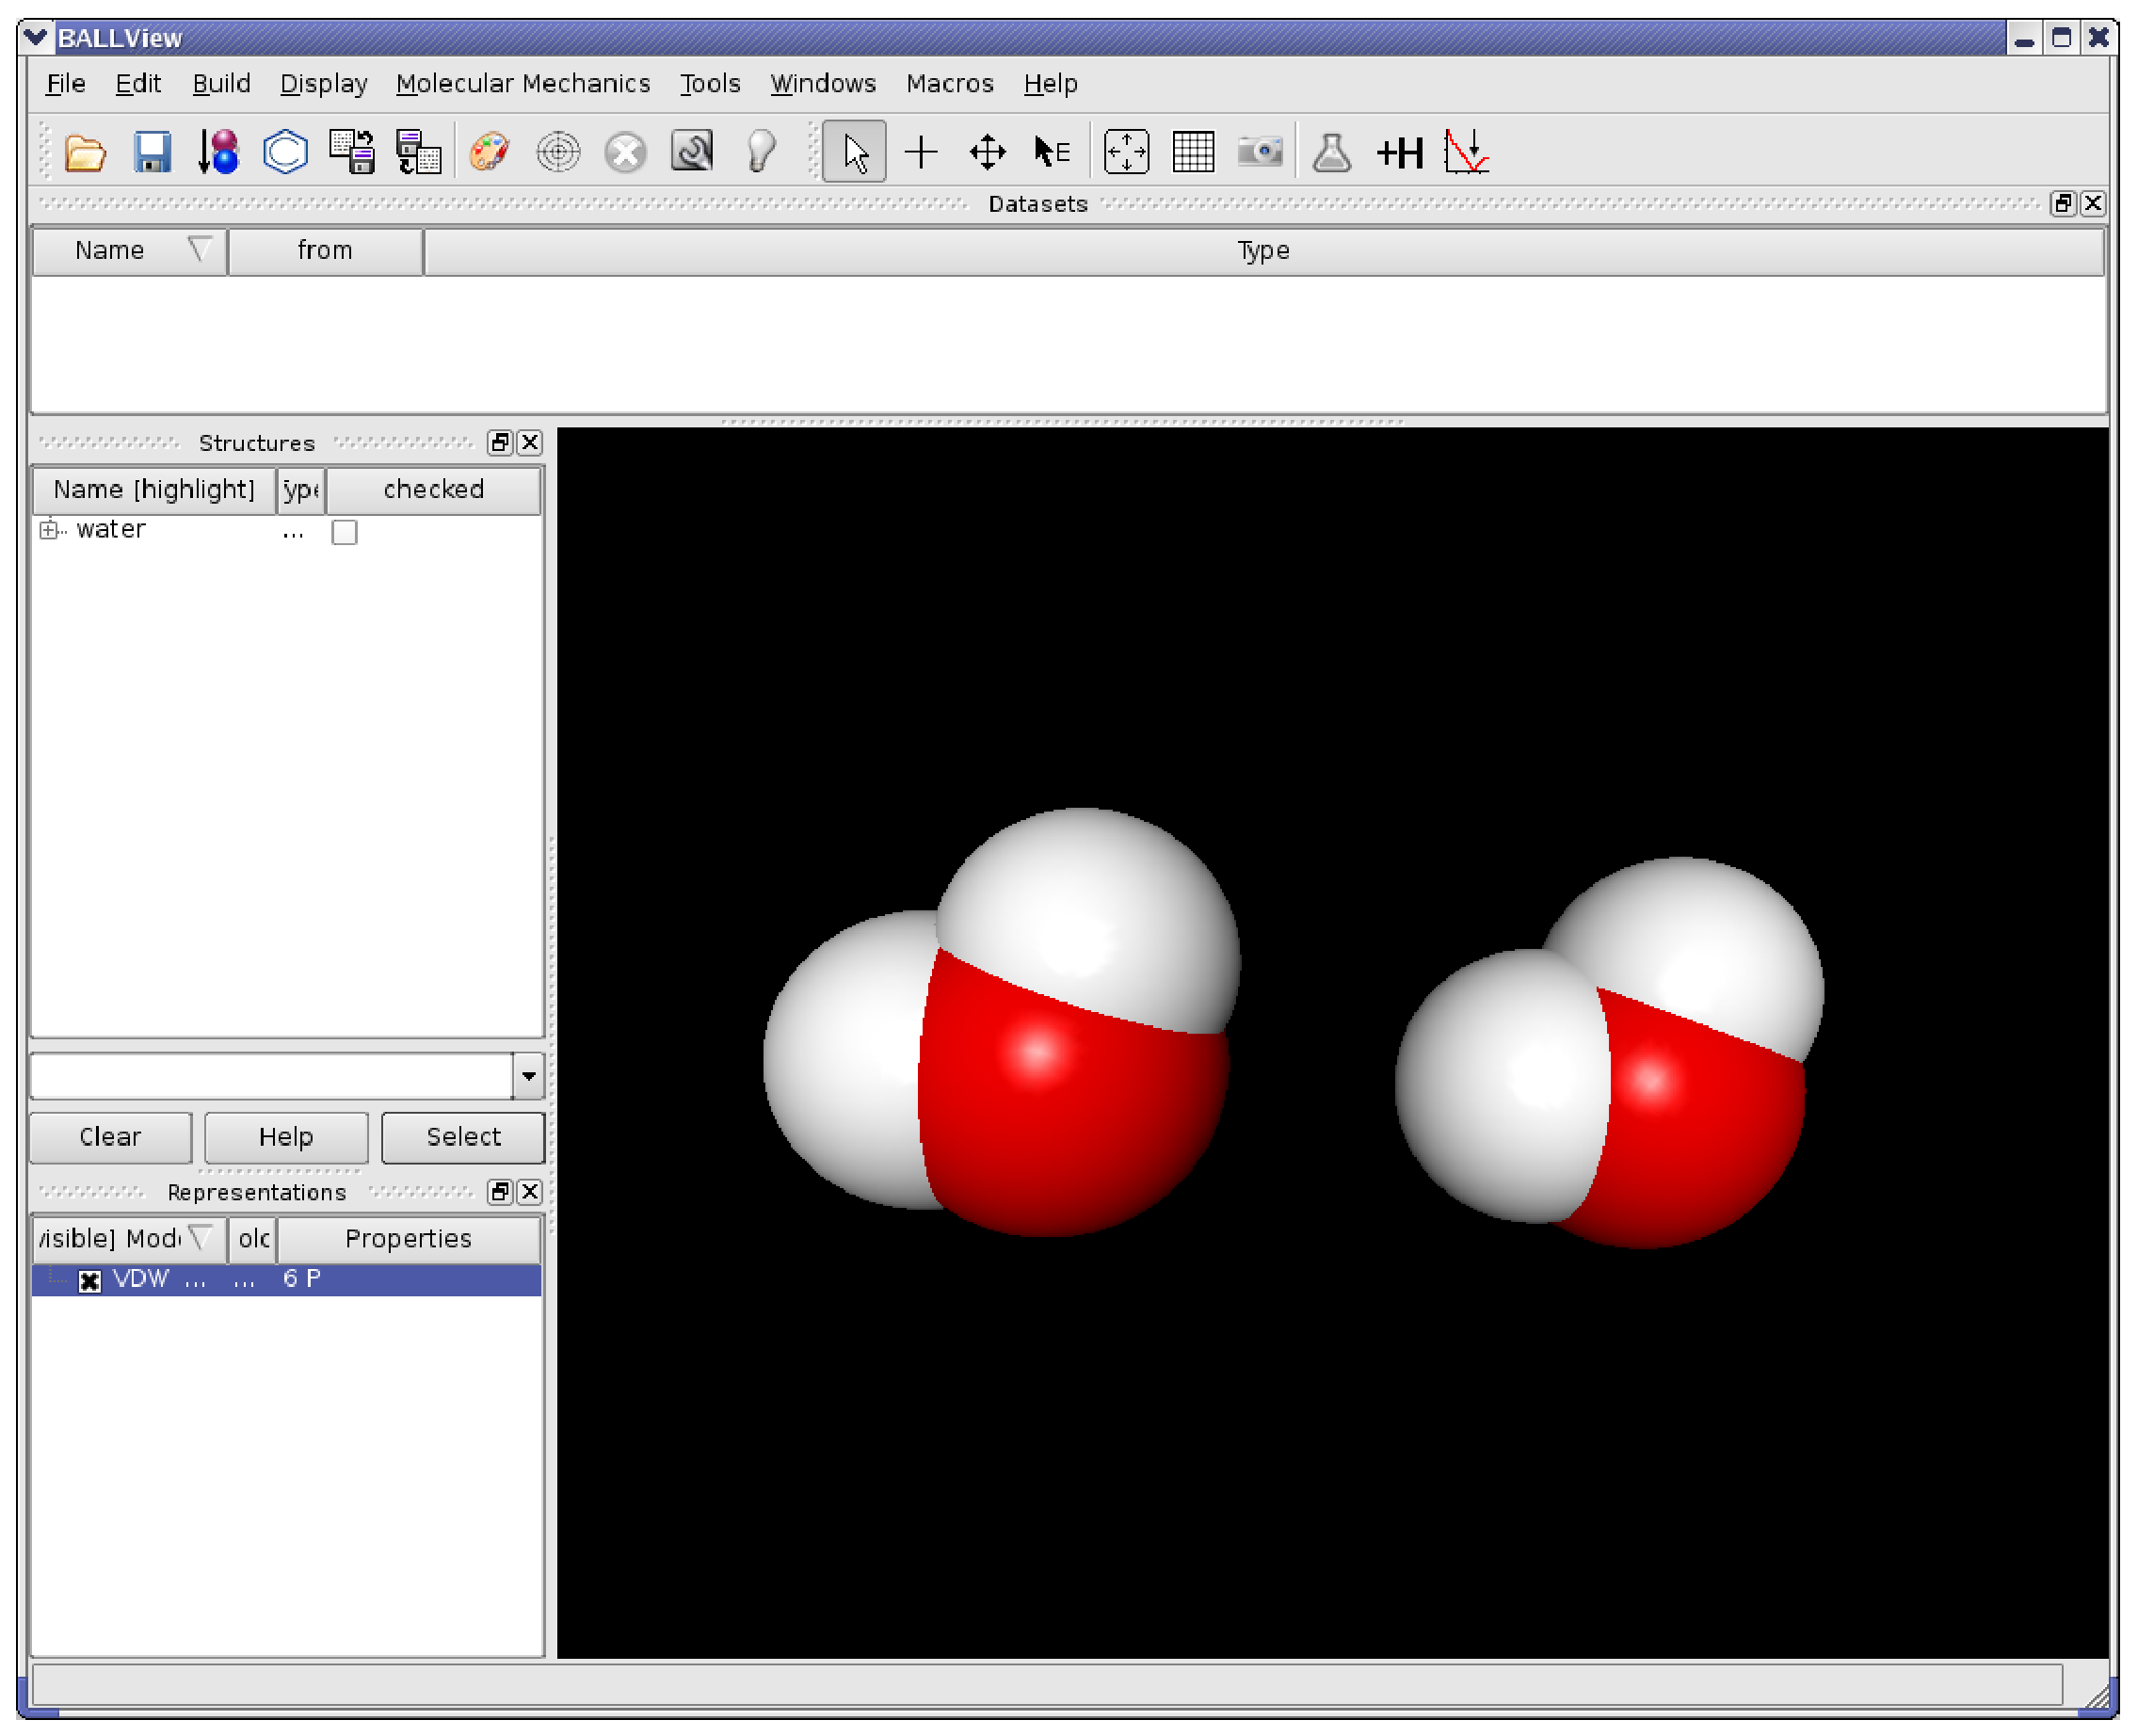
\includegraphics[width=\textwidth]{tut1_screenshot}
  \caption{Screenshot of BALLView showing the result of the first example
           ({\tt tutorial1.C})}
  \label{fig:tut1-screenshot}
\end{figure}

\noindent
We can now manipulate the two water molecules simultaneously. For example a
further application of the translation processor to the system would apply
the translation to both molecules.
But now we would like to have a look at what we built. So we might write our
system to a file and inspect it with a molecule viewer (\eg BALLView).
BALL supports a variety of file formats. For example we could write the system
to a HyperChem HIN file~\cite{HyperChem}: \label{useofstreams}

\begin{lstlisting}{}
  HINFile outfile("water.hin", std::ios::out);
  outfile << S;
  outfile.close();
\end{lstlisting}

\noindent
These three lines of code create a \class{HINFile} object which is used to
read and write HyperChem files. The first line opens a file named {\tt
water.hin} for output ({\tt std::ios::out}; if the second argument is omitted the
file is opened for reading only). The second line uses the stream operator 
{\tt <<} \index{operator {\tt <<}} to write the contents of system {\tt S} to 
this file. The file is closed in the third line.

\noindent 
As all molecules and atoms we created are inside the system, they are deleted
automatically as soon as the system is deleted.

If this short program is run it creates the following output:

\begin{lstlisting}[frameround=]{}
  # of atoms in water: 3
  # of bonds of oxygen: 2
  # of bonds of hydrogen1: 1
  # of bonds of hydrogen2: 1
  bond distance: 0.95
\end{lstlisting}

\noindent
It also creates a file named {\tt water.hin} which contains the two water
molecules. Fig.~\ref{fig:tut1-screenshot} shows the contents of this file
in the BALLView viewer.

To compile this small example, we still have to include a few header files.
The complete file is shown in Listing~\ref{lst:tutorial1} on
Page~\pageref{lst:tutorial1} and can be found in \mbox{{\tt
BALL/source/TUTORIAL/tutorial1.C}}.

First, we have to include \file{iostream} as we use {\tt cout} and {\tt endl}
to print some text. Then, we have to include the headers for the BALL kernel
classes \class{Atom}, \class{Bond}, \class{Molecule}, \class{System}, and
\class{PTE}. The headers for the HyperChem file support are found in the
directory \directory{BALL/FORMAT} and the headers for the
\class{TranslationProcessor} class are found in
{\tt BALL/STRUCTURE/geometricProperties.h}.

As all BALL classes are hidden in the \namespace{BALL} namespace, we have to
give access to this namespace with the command 
\begin{lstlisting}{}
  using namespace BALL;
\end{lstlisting}
Similarly, we also use the namespace \namespace{std} which contains {\tt cout}
and {\tt endl}.

If you have BALL installed, you might now try to compile this example. Simply
change to the directory \directory{BALL/source/TUTORIAL} which contains all
the examples from this tutorial and type 
\begin{lstlisting}[frameround=]{}
  make tutorial1
  ./tutorial1
\end{lstlisting}
This should build and execute the example. Please remember to set the
environment variable {\tt LD\_LIBRARY\_PATH} to the directory where your
libraries are installed.

After the successful execution of the example, a file named {\tt water.hin}
should appear in the current directory. This file contains the two water
molecules. You might inspect it with the molecule viewer \mbox{BALLView}.
Fig.~\ref{fig:tut1-screenshot} shows a screenshot of \mbox{BALLView} 
displaying the two water molecules.

\newpage
\begin{lstlisting}[captionpos=t,caption={The complete source code of the first example.}\label{lst:tutorial1}]{}
// tutorial example 1
// ------------------
// build two water molecules and write them to a file

// needed for cout
#include <iostream>

// the BALL kernel classes
#include <BALL/KERNEL/atom.h>
#include <BALL/KERNEL/bond.h>
#include <BALL/KERNEL/molecule.h>
#include <BALL/KERNEL/system.h>
#include <BALL/KERNEL/PTE.h>

// reading and writing of HyperChem files
#include <BALL/FORMAT/HINFile.h>

// the TranslationProcessor
#include <BALL/STRUCTURE/geometricTransformations.h>

// we use the BALL namespace and the std namespace
using namespace BALL;
using namespace std;

int main()
{
  // we create a new atom called oxygen
  // and set its element to oxygen (PTE[Element::O])
  Atom* oxygen = new Atom;
  oxygen->setElement(PTE[Element::O]);

  // now we create two hydrogen atoms...
  Atom* hydrogen1 = new Atom;
  Atom* hydrogen2 = new Atom;
  hydrogen1->setElement(PTE[Element::H]);
  hydrogen2->setElement(PTE[Element::H]);

  // ...and move them to approximately correct positions
  hydrogen1->setPosition(Vector3(-0.95, 0.00, 0.0));
  hydrogen2->setPosition(Vector3( 0.25, 0.87, 0.0));

  // We create our water molecule...
  Molecule* water = new Molecule;

  // ...and insert the three atoms into the molecule.
  water->insert(*oxygen);
  water->insert(*hydrogen1);
  water->insert(*hydrogen2);

  // Then we build the two O-H bonds
  oxygen->createBond(*hydrogen1);
  oxygen->createBond(*hydrogen2);

  // Some statistics: Molecule::countAtoms() 
  // returns the number of atoms, Atom::countBonds() 
  // the number of bonds the atom shares
  cout << "# of atoms in water: " 
       << water->countAtoms() << endl;
  cout << "# of bonds in oxygen: " 
       << oxygen->countBonds() << endl;
  cout << "# of bonds of hydrogen1: " 
       << hydrogen1->countBonds() << endl;
  cout << "# of bonds of hydrogen2: " 
       << hydrogen2->countBonds() << endl;

  // compute the bond length
  float distance = oxygen->getDistance(*hydrogen1);

  cout << "bond length: " << distance << endl;

  // Now we copy our molecule using a copy constructor.
  Molecule* water2 = new Molecule(*water);

  // A translation processor moves the second molecule
  // 5 Angstrom along the x axis
  TranslationProcessor translation(Vector3(5, 0, 0));
  water2->apply(translation);

  // We insert our two molecules into a system
  System* S = new System;
  S->insert(*water);
  S->insert(*water2);

  // and write this system to a HyperChem file
  HINFile outfile("water.hin", std::ios::out);
  outfile << *S;
  outfile.close();

  // We delete the system. This also deletes 
  // the molecules and the atoms therein
  delete S;
}
\end{lstlisting}

\section{Handling proteins}

In the second example we take a step towards real world applications. Instead
of constructing our own molecules, we now read a protein from a \newterm{PDB
file}. The PDB format~\cite{PDB} is a standardized file format for molecular structure
data. In our case, we will read BPTI (bovine pancreatic trypsin inhibitor), a
small protein:

\begin{lstlisting}{}
	PDBFile infile("bpti.pdb");
	System S;
	infile >> S;
	infile.close();
\end{lstlisting}

\noindent
In the first line, we create a \class{PDBFile} object and assign it to a file
named {\tt bpti.pdb}. Then we create an empty system {\tt S} and read the
contents of the PDB file into the system using the stream operator {\tt >>}.
This use of the stream operators is possible for all file formats in BALL (see
also the first example). Hence, you can easily switch file formats
by changing just the type of the {\tt infile} object (\eg replace it by
\class{HINFile} to read HyperChem files).

We can now verify whether the file was correctly read. BPTI should have 594
atoms. The number of atoms in any kernel object that might contain atoms (\ie
all classes that are derived from \class{BaseFragment}) is obtained by calling
\method{countAtoms}:

\begin{lstlisting}{}
	cout << "# of atoms in BPTI: " << S.countAtoms() << endl;
\end{lstlisting}

Now, we are interested in the sequence of BPTI. Since BPTI contains only a
single chain, we might just traverse all residues of this chain and write
their names to {\tt cout}. This is done by \newterm{iterators}. Iterators are
objects that can be used to traverse container objects (\eg lists, arrays, or
-- in our case -- proteins). Iterators ``point'' to an element of a container
object. They may be incremented to get the next element and they may be
derferenced similar to pointers by using {\tt *} or {\tt ->}. In fact,
C pointers can be thought of as iterators.
The use of iterators in BALL is similar to the
use of iterators in the \newterm{Standard Template Library} (\Index{STL}).
But there is a significant difference. STL containers usually contain objects of
one single type (\eg a list of strings). In BALL kernel objects, this is
different. A system may contain atoms, proteins, molecules, residues, \etc
This leads to a difference in the interface. A typical {\tt for} loop using STL
iterators to access all elements of a list looks as follows:

\begin{lstlisting}{}
	list<string> string_list = ...;
	list<string>::iterator list_it;
	
	for (list_it = string_list.begin(); 
			 list_it != string_list.end();
			 ++list_it)
	{
		cout << *list_it << endl;
	}
\end{lstlisting}

\noindent
Here, we use a list iterator ({\tt list\_it}) to traverse the whole list ({\tt
string\_list}). The method {\tt begin()} returns an iterator that points to
the first element of the list. In the {\tt for} loop we increment the iterator
until it equals the iterator returned by {\tt end()}. This method returns a
past--the--end iterator, \ie the iterator points beyond the last element of
the container. In the body of the {\tt for} loop, we access the list element
the iterator points to using the {\tt *} operator.

Traversing a BALL kernel data structure is as simple as traversing a list with
STL. But since kernel objects may contain objects of a variety of types,
we have to define over which objects we intend to iterate.
For example iterating over all residues of our system requires a
\class{ResidueIterator}. Clearly, we also need different {\tt begin()} and
{\tt end()} methods for all data types. Hence, the loop that prints the
sequence of our protein reads as follows:

\begin{lstlisting}{}
	ResidueIterator res_it;
	for (res_it = S.beginResidue(); 
			 res_it != S.endResidue();
			 ++res_it)
	{
		cout << res_it->getName() << endl;
	}
\end{lstlisting}

\noindent
This loop iterates over all residues in {\tt S} and uses the method {\tt
Residue::}\method{getName()} to access the residues name. All proteins and
residues are traversed in the order in which they appear in the PDB file.
Since the PDB format requires the residues to start with the N-terminus,
the sequence is printed  in the correct order (N-terminus to C-terminus).

\section{A simple AMBER calculation}

Having introduced the basic of handling proteins in the last
chapter, we now turn towards real-life examples: getting a protein
from the PDB and performing an AMBER calculation with it.
Again, we will be using BPTI. Instead of reading BPTI from a 
file, as in the last example, we will use the TCP transfer
capabilities of BALL to retrieve the file directly form the 
PDB (if your machine is connected to the internet -- you might
want to read it from a file as in the last example otherwise).
All classes handling file I/O in BALL are derived from a common
base class, \class{File}. This base class provides a lot of
functionality that applies to all derived classes as well.
On eof the most usefult features is on-the-fly file transformation.
Iin our case, we can open a file (e.g. a PDB file using the \class{PDBFile} 
class) that is not stored locally on a disc, but in the internet:

\begin{lstlisting}{}
	PDBFile infile("ftp://ftp.rcsb.org/pub/pdb/data/structures/all/pdb/4pti.brk");
	System S;
	infile >> S;
	infile.close();
\end{lstlisting}

\noindent
This command retrieves the file {\tt 4pti.brk} from its location at the RCSB
site using the FTP protocol and reads the contents of that file into a
\class{System}. The retrieval and the expansion of the URL into something
meaningful is performed by the classes \class{TransformationManager} and
\class{TCPTransfer}. The transformation manager also allows you to define 
external programs that can act as a filter for reading files. For example,
you might want to store compressed files (using GNU gzip) of the PDB
instead of the uncompressed files. This is easily achieved by the simple
method call 

\begin{lstlisting}{}
	File::registerTransformation(".*\.gz", "exec:/usr/local/bin/gunzip -c %s");
\end{lstlisting}

\noindent


\chapter{Foundation Classes}
\label{chapter:foundation-classes}
\label{section:kernel-data-structures}

\noindent
The BALL foundation classes are a collection of useful classes used throughout
the whole BALL kernel. The following sections shall help you to get acquainted
with some of the more important ones. The foundation classes can be broken down
into several categories:
\begin{itemize}
  \item general data structures (\eg strings, portable data types, hash
	containers)
  \item concepts (\eg management of properties, object persistence)
  \item mathematical data structures (\eg vectors, matrices, geometric
        primitives)
  \item system classes (file I/O, networking, logging)
  \item miscellaneous other stuff (plugins)
\end{itemize}
These classes implement a plethora of useful things, so you should just browse
through the reference manual to figure out which ones suit your needs. 

Some of the classes are of fundamental importance, so we will give a short
overview of their basics in the following sections. However, the total number
of classes is too large to cover here. Please have a look at the headers in 
\directory{BALL/include/BALL/COMMON|CONCEPT|SYSTEM|MATHS|DATATYPE} and the
BALL reference manual -- it's worth the time!

\section{The BALL File Class}

All classes handling file I/O in BALL are derived from a common
base class, \class{File}. This base class provides a lot of
functionality that applies to all derived classes as well.
On eof the most usefult features is on-the-fly file transformation.
For example, we can open a file (e.g. a PDB file using the \class{PDBFile} 
class) that is not stored locally on a disc, but in the internet:

\begin{lstlisting}{}
	PDBFile
	infile("ftp://ftp.rcsb.org/pub/pdb/data/structures/all/pdb/pdb4pti.ent");
	System S;
	infile >> S;
	infile.close();
\end{lstlisting}

\noindent
This command retrieves the file {\tt pdb4pti.ent} from its location at the RCSB
site using the FTP protocol and reads the contents of that file into a
\class{System}. The retrieval and the expansion of the URL into something
meaningful is performed by the classes \class{TransformationManager} and
\class{TCPTransfer}. Any filename is first handed to the static instance of
\class{TransformationManager} \class{File} possesses, which then applies all
matching rules to that file name. The resulting expanded file names are then 
checked for special prefixes by \class{File}:
\begin{itemize}
	\item a file name starting with {\tt exec:} will execute the command after the
					colon, redirect the output of the command to a temporary file, which 	
					is the opened and returned
	\item a file name starting with {\tt http:} or {\tt ftp:} will initiate
					an HTTP or FTP tranfer from the given URL to a temporary file, which
					is opened and returned
\end{itemize}

\noindent 
THe {\tt exec:} prefix can be used to filter existing files through a command, 
e.g. the compressed (GZIPped file) {\tt test.txt.gz} can be achieved through
the filename {\tt exec:gunzip -c test.txt.gz}, assuming that the gunzip
executable is in your path. You can also automate this process using the
TransformationManger. Simply by defining a rule for all files ending in {\tt
.gz}, gunzip will be called automatically:

\begin{lstlisting}{}
	File::registerTransformation(".*\.gz", "exec:/usr/local/bin/gunzip -c %s");
\end{lstlisting}

\noindent
Similarly, if you store a local copy of the PDB in {\tt /local/PDB}, you might
want to define a short-hand for the path to the PDB through the following
rule:

\begin{lstlisting}{}
	File::registerTransformation("PDB:.*", "/local/PDB/structures/all/pdb/pdb%b.ent");
\end{lstlisting}

\noindent
This rule would then expand the name {\tt PDB://4pti} to the local copy
in {\tt /local/PDB/structures/all/pdb/pdb4pti.ent}. In the above rule, 
{\tt %b} corresponds  to the basename of the file, \ie the name without path 
and without the file type extension (everything after the last dot).
For details on the formulation of rules, please refer to the section
covering \class{TransformationManager} in the BALL Reference Manual.

Some restrictions apply when using transformed file names. First, they may
be used for {\em reading} files only -- there is no destinct rule set for
writing files. Second, te transformation manager will alway sapply the first 
rule he finds. Therefore chaining of rules is not possible and the user
is responsible for avoiding ambiguities between multiple defined rules.

\section{BALL Strings}

BALL provides a heavy-weight string class that has been designed
to provide a wealth of functionality using a simple and consistent syntax.
In general, you should avoid using {\tt const char*} or STL string when using
BALL, although they are compatible to each other. You can easily convert BALL
strings to char pointers (using the {\tt c\_str()} method and automatically
convert char pointers to BALL strings.

This part of the tutorial will give a short introduction to the wealthy
functionality of BALL strings. For complete information refer to the BALL
Referenced Manual.

\subsection{String Operations}

There are useful operations possible with BALL strings. Let us start with a
very basic one, concatenation. The following code snippet will concatenate two
BALL strings:
\begin{lstlisting}{}
String A("Concat");
String B("enate");
String C = A + B;
\end{lstlisting}
But concatenation is also defined with STL strings and even standard C
strings, \ie {\tt char*}, as operands:
\begin{lstlisting}{}
string A("Concat");
char* B = "enate";
String C = A + B;
\end{lstlisting}

Another very useful operation is swapping two strings:
\begin{lstlisting}{}
String A("Swap");
String B("swaP");
A.swap(B);
\end{lstlisting}

Something we might also use very often is reversing a string:
\begin{lstlisting}{}
String A("Swap");
A.reverse();
\end{lstlisting}

And finally, it is even possible to substitute parts of a string with another
String by using the \method{substitute} method:
\begin{lstlisting}{}
String A("Please replace REPLACE with something else.");
String B("REPLACE");
String C("SOMETHING ELSE");
A.substitute(B, C);
\end{lstlisting}


\subsection{Conversion}

BALL strings are featured with many conversion mechanisms. They are either
implemented through constructors or by one of the many explicit conversion
methods available. We will first have a look at some constructors taking other
types as argument. Let us first construct a String from some basic C types:
{\tt char}:
\begin{lstlisting}{}
char c_char = 'B';
int c_int = 1;
float c_float = 2.99792458;

String A(c_char);
String B(c_int);
String C(c_float);
\end{lstlisting}
There are many other simple types supported, like {\tt unsigned int}, {\tt
double}, etc. Refer to the reference manual for further information.

Let us turn to explicit conversions. 

\subsection{Predicates}

BALL Strings provide many predicates that can be used for determining special
properties. One ca find out, whether a String contains a certain substring, 
starts with a special prefix, ends with a suffix, consists only of letters or 
is simply a floating point number. The following code snippet will give you
some idea of the power of the predicates.

\subsection{Comparing Strings}

Commonly one often wants to compare strings, which was a pain with C type
character fields. BALL strings provide you with a simple interface and rih
functionality. 

%\include{exceptions}???
%\include{logstream}???

\chapter{Kernel}
\label{chapter:kernel}
The BALL kernel data structures have been designed to model the problem 
domain (\ie well-known biochemical entities) as closely as possible.
Although some of the terms in biochemistry are rather fuzzy, there is a clear
hierarchical relationship (Fig.~\ref{figure:problem-domain}).
BALL tries to model this hierarchical relationship as a tree structure.
The design pattern used to implement this tree is the {\em composite
pattern}\cite{DesignPatterns}, which is implemented in the \class{Composite} class.
Derived from Composite are \class{AtomContainer}, the base class of all
classes handling atoms and \class{Atom}. As a typical user, you will probably
have to use only derived classes of \class{AtomContainer}, atoms, and bonds.
The kernel classes decompose into three frameworks: the general molecular
framework, the protein framework, and the nucleic acid framework
(Fig.~\ref{figure:kernel-frameworks})
Each of these frameworks contains a few classes which try to model the
respective problem domain as closely as possible. We will briefly discuss the
roles of each of these classes before describing some of the general features
of the kernel classes.

\begin{figure}[tb]
  \centering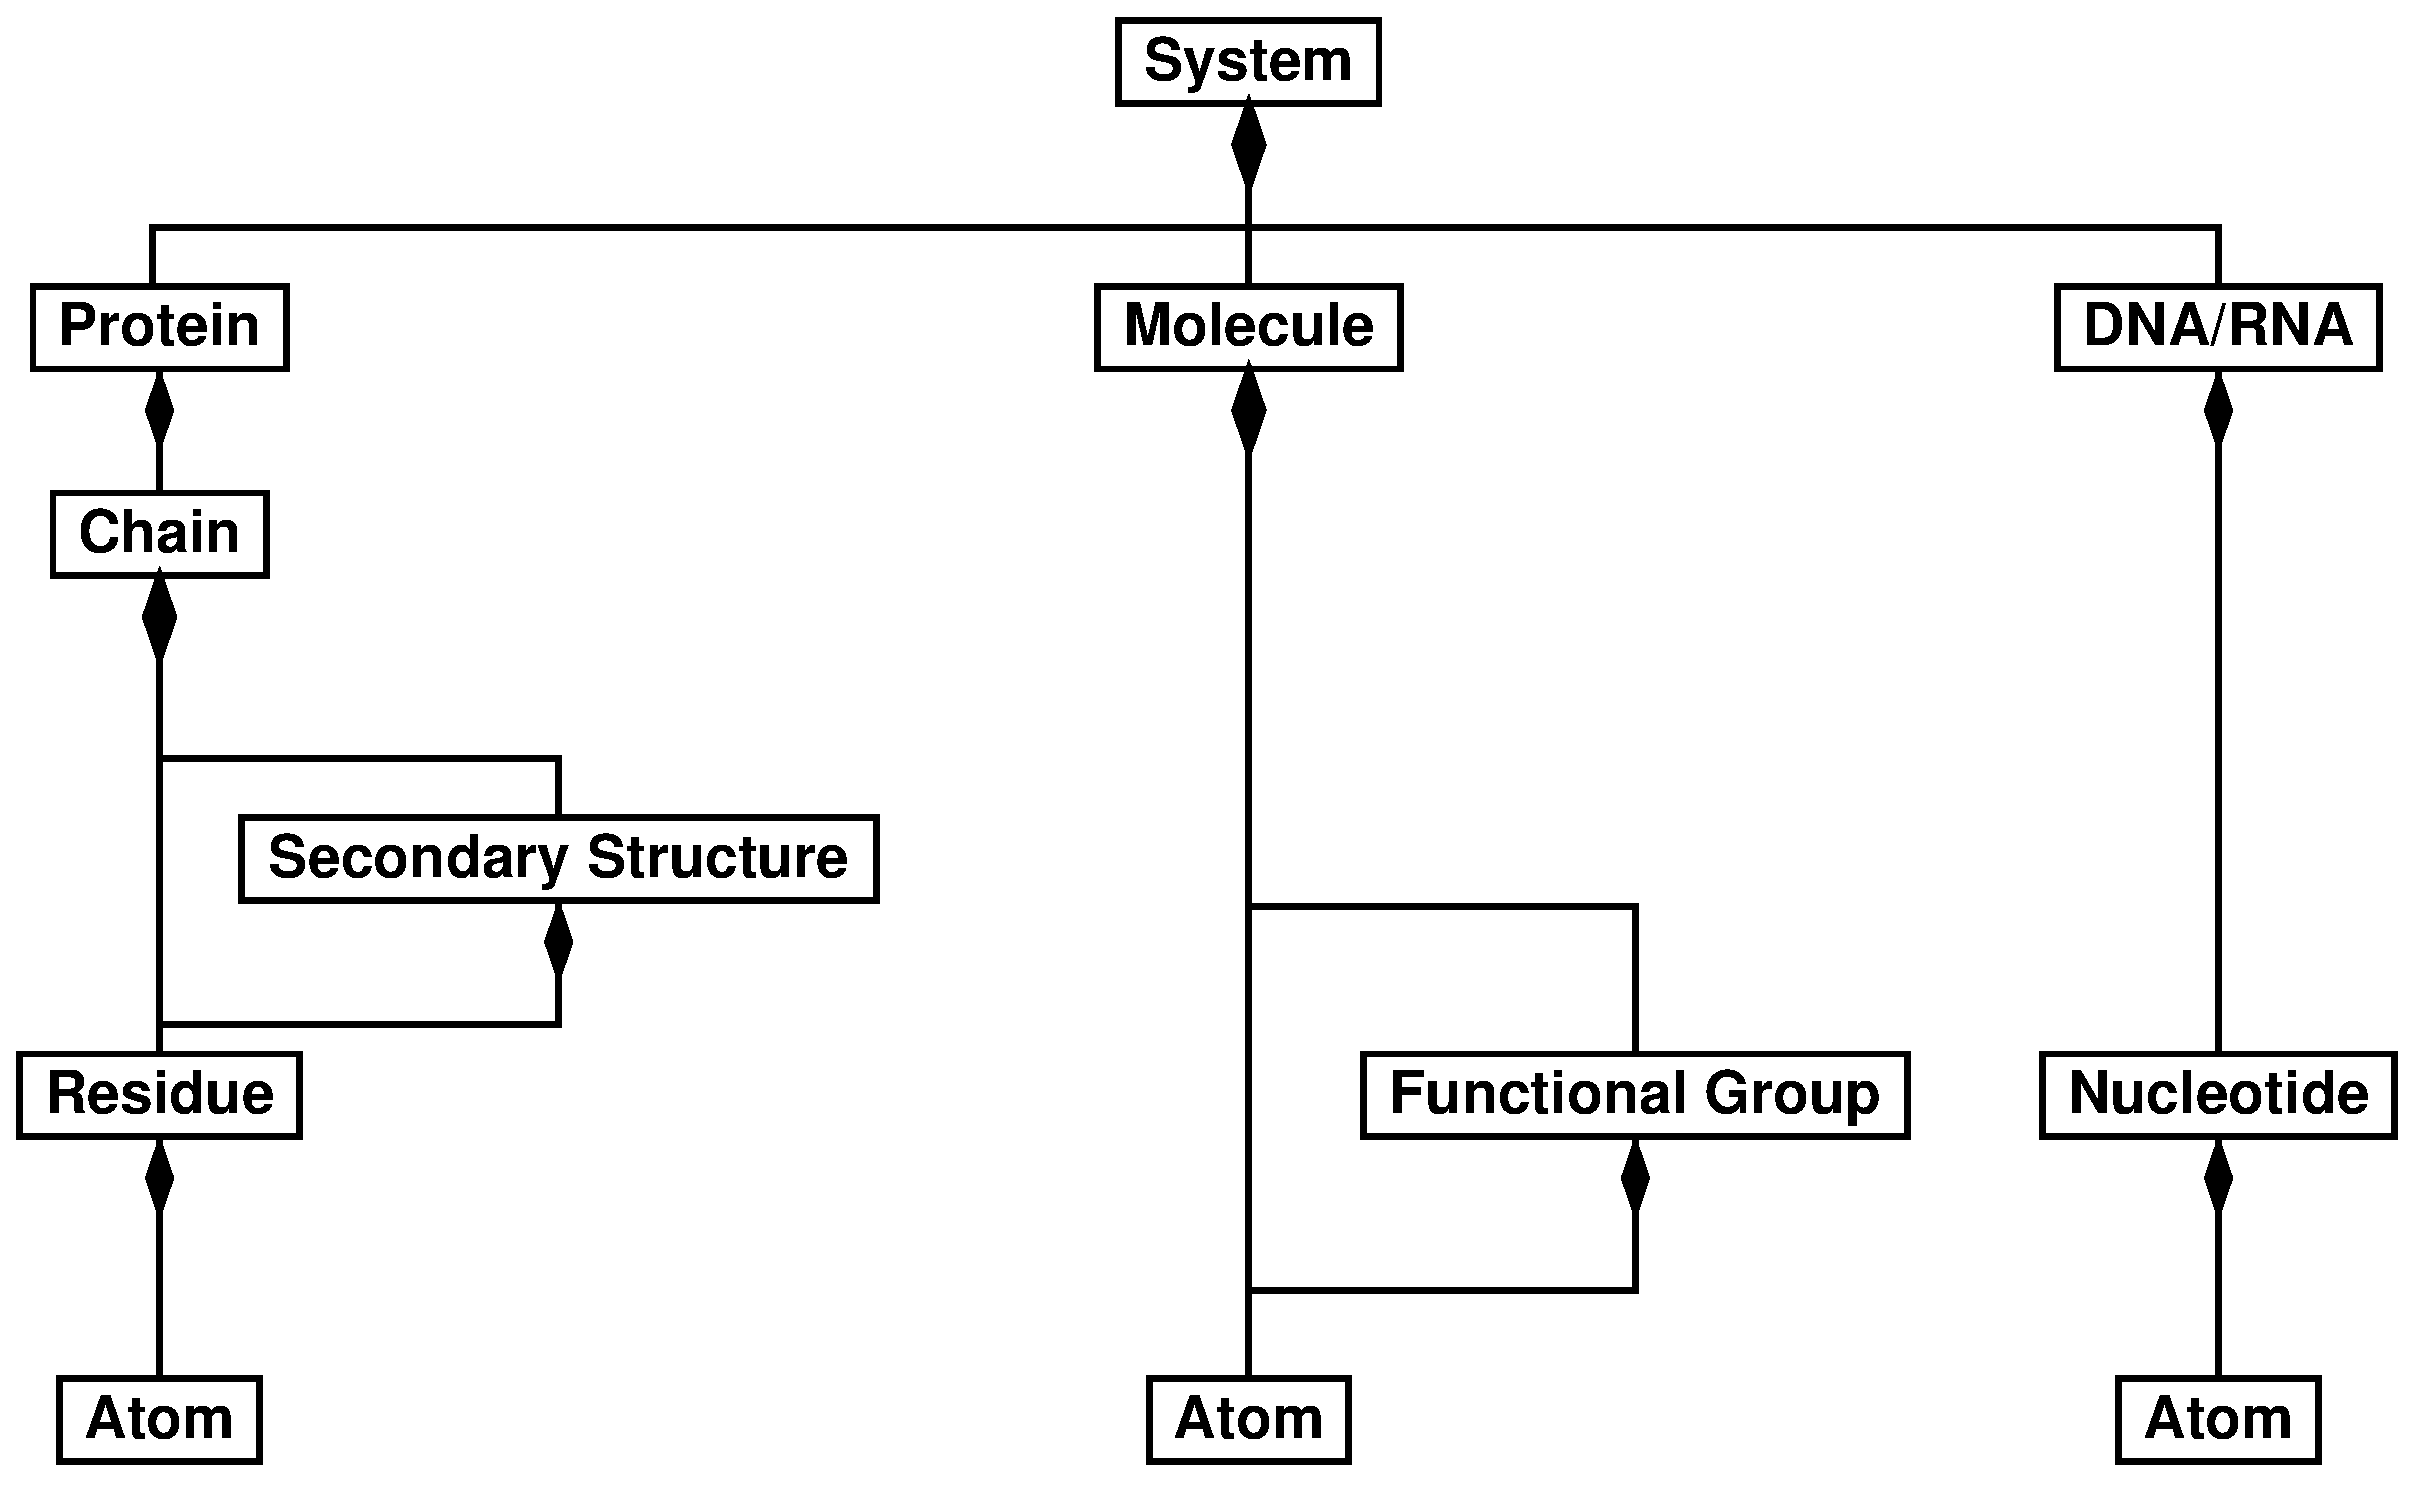
\includegraphics[width=\textwidth]{problem-domain.eps}
  \caption{A model of the biochemical problem domain. BALL tries to model
					these entities as closely as possible with its kernel classes.}
  \label{figure:problem-domain}
\end{figure}

\begin{figure}[tb]
  \centering\includegraphics[width=\textwidth]{kernel-data-structures.eps}
  \caption{The BALL kernel classes consist of three main frameworks: the
molecular framework, the protein framework, and the nucleic acid framework.}
  \label{figure:kernel-frameworks}
\end{figure}

\paragraph{The molecular framework} contains the classes \class{System},
\class{Molecule}, \class{Fragment}, \class{Bond}, and \class{Atom}. 
Molecules can contain an arbitrary number of atoms or fragments. A fragment
can be used to define distinct groups in a molecule, \eg functional groups or
charge groups. Fragments can be nested, so you may want to define several
functional groups within one larger fragment in a molecule. The atoms are then
contained in the fragments. In contrast to other systems, the atoms of a
molecule are not necessarily connected to each other (or in graph-theoretical
terms: they do not have to represent a connected component of the graph
formed by atoms and bonds). Systems are nothing but collections of molecules.

\paragraph{The protein framework} is a specialization of the general molecular
framework and describes the structures encountered in proteins. Proteins are
(more or less) molecules, so \class{Protein} is a subclass of \class{Molecule}
and proteins can be handled like molecules and stored along with them in
systems. Proteins can often be decomposed into several chains. These chains in
turn can contain secondary structure elements, which then contain residues.
Residues usually describe the amino acids of a protein. The sequence
information of a protein is encoded implicitly in the order of the tree: it
can be obtained by reading all instances of \class{Residue} in the order they
are contained in a protein. So the protein, the chains, and secondary
structure elements should contain the residues in the correct order, from
N-terminal to C-terminal, if you construct them by hand. The first and last
residue of a chain are considered to be terminal (according to the member
function \member{Residue}{isTerminal}). This is also the reason why a protein
should always contain at least one chain. Secondary structure elements,
defined by \class{SecondaryStructure} are optional. Wherever this information
is known (\eg when read from PDB files), instances of
\class{SecondaryStructure} are created to store it. Each secondary structure
element contains a class {\eg helix, $\beta$-sheet) describing its type.

\paragraph{The nucleic acid framework} contains the classes \class{NucleicAcid}
and \class{Nucleotide} and is used to represent structures of nucleic acids.
Right now, we do not differentiate between DNA and RNA, so if you need these
classes, we are eager to get your input on how to model DNA and RNA in a more
detailed way -- currently do not have yet any application for it.

By deriving all kernel classes from the common base class \class{Composite},
they share all the features implemented there. The following section will
briefly discuss some of these features.

\paragraph{Iteration} over kernel data structures is a key concept in BALL.
The BALL kernel iterators a re STL-like iterators. Since most BALL kernel
classes are so-called {\em multi-containers}, \ie they can contain different
objects, we cannot use the typical STL {\tt begin()}/{\tt end()} methods.
For example in a protein, you might not only want to iterate over all chains,
but also over all residues or all atoms contained therein. So in BALL there
are the methods \member{System}{beginChain()}/


\chapter{VIEW Programming}
\label{chapter:view-programming}

This tutorial will show you how to implement geometric primitives and dialogs/widgets.
In VIEW there are a number of predefined geometric primitives already available,
e.g. {\em GLSphere}, {\em GLTube} etc. More often there is the case that a needed
primitive is not available and therefore must be programmed anew. The first part
of this tutorial will show how this is achieved. A new primitive, the cross, will
be introduced.\\
Another crucial step in implementing an application is the programming of
dialogs or widgets, their interaction with the other widgets and the integration into
the main application. In the second part we will discuss the creation of a dialog 
that will have all the above properties.

\section{How to create a geometric primitive}
\label{section:view_create_a_geometric_primitive}

In this section we want to create a new geometric primitive called 'cross'.
A cross is a shape that consists of three lines that merge in one point.
The lines are each axis aligned and meet each other in the middle.
To accomplish this we need three additional properties for the geometric object:
first the class {\em Radius} that describes the half length of each line,
second the class {\em Vertex} for the middle point of the geometric primitive
and third the class {\em ColorExtension} which contains methods for changing
the color of the cross.
In addition to these classes we need the main base classes for creating a geometric
primitive. These are: {\em GeometricObject} which implements the interface each
geometric shape must have and {\em GLObject} which is needed because of the drawing
methods that must be overridden.\\
The implementation of the class GLCross follows (includes are omitted):

\begin{lstlisting}{}
class GLCross: 
	public GeometricObject,
	public ColorExtension,
	public Radius,
	public Vertex,
	public GLObject
{
public:

	GLCross() {}
	virtual ~GLCross() {}

protected:

	virtual bool draw(bool with_names = false);
};
\end{lstlisting}

The copy constructor and the copy assignment methods have been omitted because
they are not crucial to the implementation of a primitive. 
We have a closer look to the implementation of the drawing method.
We use OpenGL code in this method to create the cross.

\begin{lstlisting}{}
bool GLCross::draw(bool with_names)
{
	if (hasProperty(GeometricObject::PROPERTY__OBJECT_HIDDEN))
		return true;
\end{lstlisting}

If the property of the primitive is set to {\em PROPERTY\_\_OBJECT\_HIDDEN} than
do not draw it. 

\begin{lstlisting}{}
	if (isSelected() == false)
		glColor4ub((unsigned char)getColor().getRed(),
							 (unsigned char)getColor().getGreen(),
							 (unsigned char)getColor().getBlue(),
							 (unsigned char)getColor().getAlpha());
	else
		glColor4ub((unsigned char)getSelectedColor().getRed(),
							 (unsigned char)getSelectedColor().getGreen(),
							 (unsigned char)getSelectedColor().getBlue(),
							 (unsigned char)getSelectedColor().getAlpha());
\end{lstlisting}

If the primitive is selected than use the selected color. Otherwise
we use the color set with the method {\em setColor}.

\begin{lstlisting}{}
	if (with_names)
		glLoadName(getGLPrimitiveManager()->getName(*this));
\end{lstlisting}

If we want to allow our primitive to be picked than we have to add this code
to the draw method. The method {\em glLoadName} is a method from the OpenGL
library. This method sets the name of the primitive so that it can be identified
later. To assure that the names are unique we use the name generating facility the class
{\em GLPrimitiveManager} provides.

\begin{lstlisting}{}
	glBegin(GL_LINES);
	glVertex3f((GLfloat)(getVertex().x - getRadius()),
						 (GLfloat)(getVertex().y),
						 (GLfloat)(getVertex().z));
	glVertex3f((GLfloat)(getVertex().x + getRadius()),
						 (GLfloat)(getVertex().y),
						 (GLfloat)(getVertex().z));

	glVertex3f((GLfloat)(getVertex().x),
						 (GLfloat)(getVertex().y - getRadius()),
						 (GLfloat)(getVertex().z));
	glVertex3f((GLfloat)(getVertex().x),
						 (GLfloat)(getVertex().y + getRadius()),
						 (GLfloat)(getVertex().z));

	glVertex3f((GLfloat)(getVertex().x),
						 (GLfloat)(getVertex().y),
						 (GLfloat)(getVertex().z - getRadius()));
	glVertex3f((GLfloat)(getVertex().x),
						 (GLfloat)(getVertex().y),
						 (GLfloat)(getVertex().z + getRadius()));
	glEnd();

	return true;
}
\end{lstlisting}

The last part of the method contains the OpenGL code for rendering the cross.
We use three lines to create the cross. All have the vertex as the middle point
and extend half the radius in each axis direction.

Now we are finished and can use the new shape by appending it to a {\em Composite}
object. It will be properly rendered.


\section{Construction of a dialog}
\label{section:view_construction_of_a_dialog}

In this tutorial we discuss the creation of a dialog. The construction of a widget
is equally easy. Just swap the base class QDialog with the base class QWidget.
That should do the trick.
The construction of a dialog/widget is somewhat complicated because of the many
actions it can perform.
A dialog can have menu entries in the main application (derived from the {\em MainControl}),
uses preferences tab widgets inserted into the {\em Preferences} dialog and can react to
messages sent from other dialogs/widgets (see {\em Message} and {\em ModularWidget}).
We want to create a dialog which have all of the above properties.\\
The menu entry our dialog should have will toggle the visibility of the dialog. Further
if the dialog is visible the menu entry will be checked, otherwise it will not be checked.
The preference tab widget has only a color control whose contents can be changed. This contents
will be written to and read from the {\em INIFile} the main application keeps.
The {\em Message} that should trigger some effect will be the message {\em SelectionMessage}
that is sent by the class {\em Control} whenever the selection changes.
To accomlish all these things we have to override certain methods and create a preferences tab
widget.\\ \\
First we have a look to the header file of our dialog (includes are omitted):

\begin{lstlisting}{}
class TestDialog: public QDialog, public ModularWidget
{
	Q_OBJECT

public:

	TestDialog(QWidget* parent = 0, const char* name = 0);
	virtual ~TestDialog() {}

	virtual void initializeWidget(MainControl& main_control);
	virtual void checkMenu(MainControl& main_control);
	virtual void finalizeWidget(MainControl& main_control);
	virtual void initializePreferencesTab(Preferences &preferences);
	virtual void finalizePreferencesTab(Preferences &preferences);
	virtual void applyPreferences(Preferences &preferences);
	virtual void fetchPreferences(INIFile &inifile);
	virtual void writePreferences(INIFile &inifile);
	virtual void onNotify(Message *message);

protected slots:
			
	void applyButtonClicked() {};
	void openDialog();

private:

	TestPreferences *test_preferences_;
	QPushButton *apply_button_;
	int id_;
	List<Composite*> selection_;
	ColorRGBA color_;
};
\end{lstlisting}

See {\em ModularWidget} for information about the various methods that must be
overridden.
Now we discuss the implementation of these methods:\\

Before we handle the initialization, update and the removal of the menu entries lets
have a look to the implementation of the constructor.

\begin{lstlisting}{}
TestDialog::TestDialog(QWidget* parent, const char* name)
	: QDialog(parent, name, FALSE, 2768)
{
	setCaption("TestDialog");
	ModularWidget::registerWidget(this);

	apply_button_ = new QPushButton(this, "apply_button");
	apply_button_->setGeometry(10, 25, 110, 30);
	apply_button_->setText( tr( "&Apply" ) );
	connect(apply_button_, SIGNAL(clicked()), 
					SLOT(applyButtonClicked()));

	color_.set("FF0000FF");
}
\end{lstlisting}

First we set the caption of this dialog than we register this dialog as a modular
widget. This action is very important because it creates the internal mechanism
that connects all widgets with each other. If you create own dialogs/widgets always
make sure this method is called.
The next thing we do is to create an apply button and connect it to our created slot
{\em applyButtonClicked}. For information about signal/slot mechanism see the QT-
library documentation.\\

In this method we create the menu entry for our dialog and connect it to a slot
that will open our dialog.

\begin{lstlisting}{}
void TestDialog::initializeWidget(MainControl& main_control)
{
	(main_control.initPopupMenu(MainControl::DISPLAY))
		->setCheckable(true);
\end{lstlisting}

First we create the menu {\em DISPLAY} if it is not already created and set
the flag {\em checkable} to assure that all entries can have a check flag.

\begin{lstlisting}{}
	id_ = main_control.insertMenuEntry
					 (MainControl::DISPLAY, "&Test Dialog", this,
						SLOT(openDialog()), CTRL+Key_T);   
}
\end{lstlisting}

Then we create the menu entry {\em Test Dialog} in the menu {\em DISPLAY}
and connect it with the slot {\em openDialog}. The id we get from this method is
stored in the variable {\em id\_}. We need this id to check the menu entry if
this dialog is open.

\begin{lstlisting}{}
void TestDialog::checkMenu(MainControl& main_control)
{
	(main_control.menuBar())->setItemChecked(id_, isVisible());
}
\end{lstlisting}

The method checkMenu is used to check or uncheck the menu entry according to the
visibility of our dialog.

\begin{lstlisting}{}
void TestDialog::finalizeWidget(MainControl& main_control)
{
	main_control.removeMenuEntry
		(MainControl::DISPLAY, "&Test Dialog", this,
		 SLOT(openDialog()), CTRL+Key_T);   
}
\end{lstlisting}

And last if the dialog is to be destroyed the menu entry will be removed from
the main application (derived from {\em MainControl}).\\

In these methods it as also possible to do other initialization or menu handling stuff.
It is even possible to add, update and remove more menu entries (for each menu entry
there must be a slot to be connected to).
For information about signal/slot mechanism see the QT-library documentation.\\

After the widget stuff we have a close look to the insertion of the preferences tab widget.
First we need a preferences tab widget.

\begin{lstlisting}{}
class TestPreferences : public QWidget
{
	Q_OBJECT
		
public:

	TestPreferences(QWidget *parent = NULL, 
									const char *name = NULL );
	virtual ~TestPreferences() {}
	
	void fetchPreferences(INIFile& inifile);
	void writePreferences(INIFile& inifile);

	ColorRGBA getColor() const { return custom_color_; }

public slots:

	virtual void editColor();

private:

	QLabel *color_sample_;
	ColorRGBA custom_color_;
};
\end{lstlisting}

In this tab widget only the contents of the color label can be changed.
This contents will be written to and read from the inifile of the main application.
This widget creates a label and an edit button. The label has no text but is
actually only a rectangle with a background color. The edit button opens a dialog
in which the color can be changed. This dialog is predefined in QT.
In the constructor we create these widgets.

\begin{lstlisting}{}
TestPreferences::TestPreferencesi
	(QWidget* parent, const char* name)
	: QWidget(parent, name, 0)
{
	QPushButton* edit_button 
		= new QPushButton(this, "edit_button");
	edit_button->setGeometry(110, 30, 80, 30);
	edit_button->setText( tr( "&Edit" ) );
	connect(edit_button, SIGNAL(clicked()), SLOT(editColor()));
\end{lstlisting}

This creates the edit button and connects it to the slot {\em editColor}.
	
\begin{lstlisting}{}
	color_sample_ = new QLabel(this, "color_sample__label");
	color_sample_->setGeometry(20, 30, 70, 30);
	color_sample_->setFrameStyle( 50 );
	
	resize(380,210);
}
\end{lstlisting}

The last initialization we perform in the constructor is the creation of the
label. Then we resize the widget to the needed size. This size is related to the
size of the {\em Preferences} dialog.
The next methods we will discuss are the methods responsible for reading and
writing the contents of this widget into the inifile.\\

This method reads the preferences from the inifile.

\begin{lstlisting}{}
void TestPreferences::fetchPreferences(INIFile& inifile)
{
	if (inifile.hasEntry("WINDOWS", "Test::color"))
	{
		custom_color_.set(inifile.getValue("WINDOWS", "Test::color"));
		color_sample_->setBackgroundColor(QColor(custom_color_.getRed(), 
																						 custom_color_.getGreen(), 
																						 custom_color_.getBlue()));
	}
}
\end{lstlisting}

If the inifile has the section {\tt WINDOWS} and the key {\tt Test::color} then
we read the contents of this key and convert it to a color which we store in the
{\em custom\_color\_} (see {\em ColorRGBA}). Additionally we set the color in the label to be displayed
in the widget.\\

To write the preferences to the inifile we override this method.

\begin{lstlisting}{}
void TestPreferences::writePreferences(INIFile& inifile)
{
	inifile.setValue("WINDOWS", "Test::color", custom_color_);
}
\end{lstlisting}

{\em Note:} It is important that the section {\tt WINDOWS} and the key {\tt Test::color} are
already inserted into the inifile else the inifile will not insert the color
into it. See {\em INIFile} for further information.\\

The last method of the preferences tab widget is the method {\em editColor} that
is called if the edit button is pressed.

\begin{lstlisting}{}
void BoundingBoxPreferences::editColor()
{
	color_sample_->setBackgroundColor(
			QColorDialog::getColor(color_sample_->backgroundColor()));
\end{lstlisting}

Here we call the dialog {\em QColorDialog} where we can change the color. If this
dialog was exited by pressing the ok button we transfer the color into the color label.

\begin{lstlisting}{}
	ColorRGBA color;
	QColor qcolor = color_sample_->backgroundColor();
	color.set((float)qcolor.red() / 255.0,
						(float)qcolor.green() / 255.0,
						(float)qcolor.blue() / 255.0);
	
	custom_color_ = color;
}
\end{lstlisting}

Now we convert the {\em QColor} into a {\em ColorRGBA} which we store in the
variable {\em custom\_color\_} so that we can access this color with the method
{\em getColor}.\\

Now that we have created the preferences tab widget we can implement the methods that 
are needed in our dialog to install this preferences tab widget.\\ 

In this method the preferences tab widget will be initialized and inserted into the
{\em MainControl}

\begin{lstlisting}{}
void TestDialog::initializePreferencesTab(Preferences &preferences)
{
	test_preferences_ = new TestPreferences();
	preferences.insertTab(test_preferences_, "TestPreferences");
}
\end{lstlisting}

We create a new {\em TestPreferences} and insert as a tab widget it into the 
{\em Preferences} dialog with name {\tt TestPreferences}.

\begin{lstlisting}{}
void TestDialog::applyPreferences(Preferences &)
{
	if test_preferences_ != 0)
		color_ = test_preferences_->getColor();
}
\end{lstlisting}

This method is called from {\em MainControl} if the apply button in the {\em Preferences} dialog
is pressed.
In this method we transfer the color from the preferences tab widget into the private
variable {\em color\_} for later usage.\\

Removal of the preferences tab widget from the {\em MainControl} and freeing of used
memory.

\begin{lstlisting}{}
void TestDialog::finalizePreferencesTab(Preferences &preferences)
{
	if (test_preferences_ != 0)
	{
		preferences.removeTab(test_preferences_);
		delete test_preferences_;
	}
}
\end{lstlisting}

This method will be called by the {\em MainControl} if the application is closed. We
remove our preferences tab widget from the preferences dialog and delete it afterwards.\\

To relay fetch and write actions to the preferences tab widget we must override
the same methods in the dialog.\\
This method reads the preferences of our dialog from the inifile and calls
the same method of the preferences tab widget.

\begin{lstlisting}{}
void TestDialog::fetchPreferences(INIFile& inifile)
{
	int x_pos = x();
	int y_pos = y();

	if (inifile.hasEntry("WINDOWS", "Test::x"))
		x_pos = inifile.getValue("WINDOWS", "Test::x").toInt();

	if (inifile.hasEntry("WINDOWS", "Test::y"))
		y_pos = inifile.getValue("WINDOWS", "Test::y").toInt();

	move(x_pos, y_pos);
\end{lstlisting}

Here we read the position of our dialog from the inifile and convert it into
integer. If the needed keys do not exist in the inifile we use the position
of our dialog (see QT-library documentation for further informations). If
we have a valid position we move our dialog to this position.

\begin{lstlisting}{}
	if (test_preferences_ != 0)
	{
		test_preferences_->fetchPreferences(inifile);
		color_ = test_preferences_->getColor();
	}
}
\end{lstlisting}

If a preferences tab widget exists we fetch its preferences from the inifile and
retrieve the color from it.\\

To write the preferences to the inifile we override this method. In this method we
write all preferences this dialog has to the inifile and call the same method
for our preferences tab widget.

\begin{lstlisting}{}
void TestDialog::writePreferences(INIFile& inifile)
{
	inifile.setValue("WINDOWS", "Test::x", String(x()));
	inifile.setValue("WINDOWS", "Test::y", String(y()));
\end{lstlisting}

With the method {\em setValue} we set the position of our dialog into the inifile.\\
{\em Note:} this method only works if the section {\tt WINDOWS} and the keys
{\tt Test::x} and {\tt Test::y} are already inserted into the inifile.

\begin{lstlisting}{}
	if (test_preferences_ != 0)
		test_preferences_->writePreferences(inifile);
}
\end{lstlisting}

If our preferences tab widget exists we write its preferences into the inifile as well.\\

The only thing that must be implemented yet is the mechanism that handles any
messages received from our dialog.
This is done in the method {\em onNotify}. 

\begin{lstlisting}{}
void TestDialog::onNotify(Message *message)
{
	selection_.clear();

	if (RTTI::isKindOf<SelectionMessage>(*message))
		selection_ = (RTTI::castTo<SelectionMessage>(*message))
										->getSelection();
\end{lstlisting}

First we clear our previously stored selection then we perform a runtime type identification
of the received message and react only if the message is of kind {\em SelectionMessage}.
	
\begin{lstlisting}{}
	if (selection_.empty())
		apply_button_->setEnabled(false);
	else
		apply_button_->setEnabled(true);
}
\end{lstlisting}

We enable the apply button in our dialog if the selection list contains any elements.
Otherwise we disable it.\\

Now we are finished with the construction of this dialog. It can be added to the main application
by creating it with a pointer to the application ({\em MainControl}) as
parent.



\chapter{BALLView Programming}
\label{chapter:BALLView-programming}
\include{BALLView}

\chapter{Python Extensions}
\label{chapter:python}
\section{Overview}
Python is an object-oriented scripting language\cite{Python} that is well
suited both as a language for embedding scripts into BALL application and as a
rapid prototyping language using the underlying BALL objects.
BALL provides Python bindings for most of its classes in order to allow Rapid
Methodology Development (RMD). Some of the functionality BALL provides (\eg
template classes, iterators) are unavailable due to the fundamental differences 
between the two languages. However, the majority of the classes is available and
workarounds exist for some of the template- and iterator-related problems.

The current Python support is not yet fully tested and debugged, therefore it
is disabled by default. If you can live with
this and think it is still a useful feature worth testing out, please read on,
otherwise pretend it doesn't exist. The remainder of this section assumes that
you are somewhat familiar with the most important language concepts of Python.

BALL relies on SIP \cite{SIP} (version 4.0 or above) to translate its class
headers semi-automatically into python wrapper classes. For each \CPP class
SIP creates a subclass defining the Python interface and a Python class
using that \CPP interface class. The Python class has the same name as the
\CPP class, so porting code from \CPP to Python (and vice versa) gets trivial.
The \CPP code 

\begin{lstlisting}{}
	System S;
	HINFile f("test.hin");
	f >> S;
\end{lstlisting}

\noindent
translates to the Python code

\begin{lstlisting}{}
	S = System()
	f = HINFile("test.hin")
	f >> S;
\end{lstlisting}

\noindent
In this example, the main difference lies in the way \CPP and Python handle
constructors. Another important difference concerns iterators. The STL-like
kernel iterators of BALL map to a set of functions (called extractors). An
extractor traverses the whole container and creates a Python sequence object
from it. Instead of havin an \class{AtomIterator} iterating over all atoms of
a residue

\begin{lstlisting}{}
	AtomIterator ai = residue.beginAtom();
	for (; +ai; ++ai)
	{
		std::cout << ai->getName() << std::endl;
	}
\end{lstlisting}
\noindent you would use the \function{atoms} extractor to create a sequence
object containing all objects of the residue in Python:

\begin{lstlisting}{}
	for atom in atoms(residue):
		print atom.getName()
\end{lstlisting}

\noindent For the template problem, we pre-instantiated some of the 
commonly used instances, \eg \class{UnaryProcessor<Atom>} maps to the 
\class{AtomProcessor} class and classes derived from it in Python.

The BALLView application contains an interactive interpreter window
if BALL was compiled with Python support. You can even access the
data structures of the viewer from there. Assuming that you are
currently displaying a structure in the viewer, you can retrieve a
reference to the first system displayed through the somewhat cryptic
command {\tt system =
MainControl::getInstance(0).getDescriptorList()[0].getComposite()}.
This is pretty useful for extracting properties from the stuff you are
currently displaying, but very deadly if you start modifying internals
of the viewer. You also should not try to destroy those objects in the
viewer, or you will be rewarded with a core dump: there is not yet
internal reference counting on the BALL side, so Python's reference
counting is nearly always wrong.
		

\section{Known bugs}
\begin{itemize}
	\item No documentation yet
	\item No unit tests yet
	\item As mentioned above, problems with reference counting.
	\item Python support requires the visualization support for some rather
				arcane internal reason we won't disclose here.
	\item {\tt configure} does not yet identify SIP and its libraries
				automatically
\end{itemize}

\section{Installation}

Donwload, configure, and install a recent version (4.0rc2 or above) of SIP from 
\URL{http://www.riverbankcomputing.co.uk/sip/}. It is important to compile SIP 
with the same \CPP compiler you compiled SIP and QT with. You can then enable the Python support of BALL
by specifying the option \mbox{"\option{--with-python=<path>}"}, where
{\tt path} should point to the executable of an installed Python (version 2.2
preferred). You will also have to specify the path to the SIP executable, its
headers, and its library ({\tt libsip.a|so}). Adding these four options might
look something like this on your system:

\begin{lstlisting}{}
	./configure \
		--with-python=/opt/bin/python2.2\
		--with-sip=/opt/bin/sip\
		--with-sip-incl=/opt/include/sip\
		--with-sip-lib=/opt/lib
\end{lstlisting}

\noindent
After configuring and building BALL, you should then change to {\tt
BALL/source/PYTHON/EXTENSIONS}. Here, you will have to run

\begin{lstlisting}{}
	make sip
	make depend
	make
	make install
\end{lstlisting}

\noindent
in order to build the Python bindings, which are then installed to {\tt
BALL/lib/<platform>}. 
You can then execute the {\tt pyball} script in {\tt
BALL/source/PYTHON/EXTENSIONS} to get an interactive Python shell with the
BALL bindings or just start the Python interpreter and import the BALL
bindings through

\begin{lstlisting}{}
	from BALL import *
\end{lstlisting}

\noindent
Note, that you have to add the directory where the bindings are installed to
Python's module search path ({\tt sys.path}).


\chapter{FAQ}
\label{chapter:faq}
\newpage
\noindent
{\it An up-to-date and searchable version of this FAQ is available at our website:\\
\FAQURL{http://www.bioinf.uni-sb.de/OK/BALL/}}\\
\hspace{1mm}
\rule{\textwidth}{0.1pt}
\hspace{3mm}
\FAQCategory{Documentation}
\FAQquestion{Are there Research reports available?}
\FAQanswer{Yes. Publications and research reports on BALL are listed on our website: 
\FAQURL{http://www.ball-project.org}
}
\FAQquestion{How do I use BALLView?}
\FAQanswer{Take a look at the builtin BALLView Tutorial or on the documentation at http://www.ball-project.org/Documentation or under BALL/doc/BALLView}
\FAQCategory{Installation}
\FAQquestion{Will BALL run on my hardware/with my compiler?}
\FAQanswer{An up-to-date list of all supported platforms can be found on the BALL website at 
\FAQURL{http://www.ball-project.org/Support/FAQ/Platforms}
}
\FAQCategory{License}
\FAQquestion{Under what kind of license is BALL available?}
\FAQanswer{
	BALL is mostly being distributed under the Lesser GNU Public License (LGPL). Parts of BALL (BALLView) are under the GNU Public License (GPL).
}



\newpage
\addtocontents{toc}{\protect\contentsline{chapter}{Index}{\thepage}}
\printindex
\renewcommand{\bibname}{References}
\addtocontents{toc}{\protect\contentsline{chapter}{References}{\thepage}}
\bibliographystyle{abbrv}
\bibliography{tutorial}

\end{document}
